%%%%%%%%%%%%%%%%%%%%%%%%%%%%%%%%%%%%%%%%%%%%%%%%%%%%%%%%%%%%%%%%%%%%%%%%%%%%%%%%
%% INTRODUCTION
%%%%%%%%%%%%%%%%%%%%%%%%%%%%%%%%%%%%%%%%%%%%%%%%%%%%%%%%%%%%%%%%%%%%%%%%%%%%%%%%

To evaluate  probabilistic properties of a software product line, reliability
in particular, initially it is necessary representing the variable behavior
jointly with the probabilistic information. Briefly, such information
represents the success and failure probabilities of executing the
communications between software components. Both behavioral variability and
probabilistic information of software product lines can be represented by the
UML activity and sequence diagrams. Later, such diagrams can be transformed
into their respective fully probabilistic models (FDTMCs), which must represent the
states variation of the context comprising all products of the software product
line. 

The software product line's behavior can be considered at two abstraction
levels. The high level is a coarse-grained representation that employs the UML
activity diagram for modeling the set of activities executed by \emph{all} products.
The low level is a fine-grained representation whose role is to model the whole
variable and probabilistic behavior of a software product line. Since the
variable behavior is defined by the interaction among software components,
such behavior is modeled by means of UML sequence diagrams. To represent the
probabilistic information of the behavior represented by both activity and
sequence diagrams, their semantics  can be extended by the UML
MARTE~\cite{uml-marte-profile} profile.  Thus, the joint representation of
behavioral variability and probabilistic information in UML behavioral diagrams
is the suitable notation for modeling the probabilistic behavior of a software
product line. 

The evaluation of software's probabilistic property consists of analyzing
whether a property specification is fulfilled in a probabilistic model. In the
case of software product lines such probabilistic model must also address the
inherent behavioral variability and the Feature Discrete-Time Markov Chain
(FDTMC) is a suitable modeling notation. As previously mentioned, an FDTMC is a
Discrete-Time Markov Chain (DTMC) endowed with variability for representing all
products' behavior (c.f. Section~\ref{subsec:featureDiscreteTimeMarkovChains}),
while the reliability property is defined as the reachability measure that
expresses the probability of reaching a set of sucessfull states on a
probabilistic model~\cite{grunske_specification_2008}. 

This chapter presents how the variable and probabilistic behavior of a software
product line can be modeled by UML behavioral diagrams (activity and sequence
diagrams) and later transformed into FDTMCs. The behavioral modeling of software
product lines is addressed in Section~\ref{sec:probabilisticVariableBehavior}
that introduces the coarse-grained behavioral representation by UML activity
diagrams (Section~\ref{subsec:umlActivityDiagrams}), followed by the
probabilistic and variable behavioral representation provided by UML sequence
diagrams (Section~\ref{subsec:umlSequenceDiagrams}).
Section~\ref{sec:reliabilityUMLBehavioralModels} introduces the reliability
notion for UML behavioral diagrams and how it is considered in the context of
software product lines. Section~\ref{sec:transformationUMLFDTMC} presents a set
of transformation rules for creating FDTMC models from UML behavioral models.
Section~\ref{sec:reliabilityEquivalenceUMLBehavioralModelsFDTMCs} demonstrates
evidences that the reliability computed based on UML behavioral diagrams and the
reliability computed based on its corresponding FDTMCs are equivalent, which
supports the correctness of transformation rules. Finally,
Section~\ref{sec:modelingConclusion} presents concluding remarks.










%%%%%%%%%%%%%%%%%%%%%%%%%%%%%%%%%%%%%%%%%%%%%%%%%%%%%%%%%%%%%%%%%%%%%%%%%%%%%%%%
%% PROBABILISTIC AND VARIABLE BEHAVIOR
%%%%%%%%%%%%%%%%%%%%%%%%%%%%%%%%%%%%%%%%%%%%%%%%%%%%%%%%%%%%%%%%%%%%%%%%%%%%%%%%
\section{Probabilistic and Variable Behavior Modeling of Software Product Lines
	\label{sec:probabilisticVariableBehavior}}

Representing the software's characteristics by models is useful to preview
and to analyze its diverse properties and behavior. Among the notations for
software representation the Unified Modeling Language (UML) stands out as it
provides manifold diagrams to address the different software's characteristics.
Within the range of UML diagrams the activity diagram is a high level and coarse-grained
behavioral representation that is usually employed to represent  the
software's main tasks and their execution order. The sequence diagram is a
fine-grained behavioral representation that details how software
components interact during a task execution. The UML MARTE profile augments the
semantics of activity and sequence diagrams by associating probabilistic
information to their behavioral elements.
%Thus, the UML behavioral diagrams
%provides different abstraction levels that allows representing which are the
%main software's tasks at first and then refine its behavioral details.

%This work is devoted to analyzing the software product line's reliability, ie.,
%the reliability of all products it may instantiate. Reliability is a software
%property computed as the reachability measure of sucessfull states of a
%probabilistic model~\cite{larsGrunske}. Such property can be also verified in
%software product lines if its inherent variability is considered during the
%property analysis. Thus, in a brief notion, computing the software product line
%reliability consists into computing the reachability measure of sucessfull
%states in a probabilistic model endowed with variability. 

The representation of the  software product line's behavior resembles the
behavioral representation of an usual software. The differences arise because the
behavioral variability inherent to software product lines must be addressed by
the same UML behavioral elements employed at ordinary software's models. In addition,
such behavioral representations must express the probabilistic information of
all products a software product line can instantiate.   In the following, each
UML behavioral element and its associated probabilistic information will be
presented in the context of software product lines modeling. 










%%%%%%%%%%%%%%%%%%%%%%%%%%%%%%%%%%%%%%%%
%% UML Activity Diagrams
%%%%%%%%%%%%%%%%%%%%%%%%%%%%%%%%%%%%%%%%
\subsection{UML Activity Diagrams' Elements \label{subsec:umlActivityDiagrams}}

The coarse-grained behavioral model of a software product line is represented
by a UML activity diagram enriched with probabilistic information in order to
represent which are the main software product line's activities and how they
are arranged and executed by \emph{all} products.  In this representation
level, common flows are the tasks sequences that all products execute, which is
not referred to the software components interactions shared by all products.
The elements considered for such modeling level are the \textit{Initial},
\textit{Activity}, \textit{Decision}, \textit{Merge} and \textit{Final} nodes.
Each element and its meaning in the context of software product line's
behavioral modeling is described in the following.
%The coarse-grained behavioral modeling is responsible to represent which are
%the main software product line's activities and how they are arranged and
%executed by \emph{all} products.
Additional constraints are represented next to the element in a gray box.


%%%%%%%%%%%%%%%%%%%%
\begin{figure}[h!]
\begin{center}
\begin{tikzpicture}
% \draw[help lines] (0,0) grid +(3, 1);
% \draw[help lines] (0,0) grid +(3,-1);
\node[adStart](start){};
\draw[thick, ->, line width=1pt] (start.east) -- node[above, draw=none]{$1.0$}
(1.0,0);
\end{tikzpicture}
\end{center}
\caption{Initial node of a UML Activity Diagram.}
\label{fig:initial_AD}
\end{figure}

\paragraph{Initial node: \label{par:initialNodeModeling}} the initial node is
represented only once in a UML activity diagram by the filled circle shown by
Figure \ref{fig:initial_AD}. It is the execution starting  point of an activity
diagram and it has only one direct sucessor element. Since the initial node does
not have any associated interaction between software components, it has no failure chances so its execution
flows directly to its immediate sucessor, that is represented by the outgoing
edge having 1.0 as probability value.


%%%%%%%%%%%%%%%%%%%%
\begin{figure}[h!]
\begin{center}
\begin{tikzpicture}
%%%%%%%%%%%%%%%%%%% HELP LINES
% \draw[help lines] (0,0) grid +(6,1);
% \draw[help lines] (0,0) grid +(6,-1);
%%%%%%%%%%%%%%%%%%% NODES
\node[fill=none, draw=none](transp1) at (-0.5,0){$\dots$};
\node[adActiv](activity) at (1.5,0) {Activity};
\node[fill=none, draw=none](transp2) at (3.5,0){$\dots$};
\node[rectangle, fill=gray!50, draw=none](constraint) at (1.5, -1) {$rActivity \in [0,1]$};

\draw[thick,->](transp1.east) -- (activity.west);
\draw[thick,->](activity.east) -- node[draw=none, auto] {$rActivity$}
(transp2.west);
\end{tikzpicture}
\end{center}
\caption{Activity node of a UML Activity Diagram.}
\label{fig:activity_AD}
\end{figure}

\paragraph{Activity: \label{par:activityModeling}}
the activity node is represented by the named rounded rectangle shown by Figure
\ref{fig:activity_AD} and it is responsible to represent a stage of the whole
behavior modelled by the activity diagram. It has an incoming and outgoing
edges to denote when its execution starts and when finishes, respectively. Each
activity comprises a set of communications among several software components
such the probability value of the outgoing edge represents the probability
which its associated behavior is executed without errors occurrences. Such
probability value is given by computing the reliability of its associated UML
sequence diagram. Since the activity's reliability depends on the computed
reliability of its associated sequence diagram and such diagram adresses the
behavioral variability of the software product line, the outgoing edge's
probability is represented by a variable defined in $[0,1]$.
%The outgoing edge's probability is represented by the $rActivity$ variable due
%its value is directly dependent on the variable behavior of the associated
%sequence diagram. 
By convention, such variable is named as the activity name with the `r' prefix
standing for ``reliability''.  

Considering the running example of Section~\ref{sec:runningExample} each
activity node represented by Figure~\ref{fig:bsnControlLoop} has its behavior
detailed by its associated
sequence diagram. In special the sequence diagrams excerpts represented by
figures~\ref{fig:oxygenationSituation} and \ref{fig:temperatureSituation} refines the ``System identifies
\underline{situation}''. Thus the reliability value assumed by the
activity and represented by the variable \emph{rSituation}, depends directly on the
reliability computed for both sequence diagrams of figures \ref{fig:oxygenationSituation} and \ref{fig:temperatureSituation}. The
way how such variable is defined and computed will be shown later, by
sections~\ref{sec:transformationUMLFDTMC} and \ref{sec:familyBasedAnalysis}.

%%%%%%%%%%%%%%%%%%%%
\begin{figure}[h!]
\begin{center}
\begin{tikzpicture}
%%%%%%%%%%%%%%%%%%% HELP LINES
% \draw[help lines] (0,0) grid + (6,1);
% \draw[help lines] (0,0) grid + (6,-1);
%%%%%%%%%%%%%%%%%%% NODES
\node[fill=none, draw=none](init) at(-0.5,0) {$\dots$};
\node[adDecis](decision)at(1,0) {};
\node[transpNode](dec1) at(2,1) {};
\node[transpNode](dec2) at(2,-1){};
\node[transpNode](decM) at(1.5, 0){$\dots$};

\node[rectangle, fill=gray!50, draw=none](constraint) at (1.0,-1.7){$\sum p_i = 1.0$};
%%%%%%%%%%%%%%%%%%% EDGES
\draw[thick, line width=1pt, ->] (init) -- (decision);
\draw[thick, line width=1pt, ->] (decision) -- node[fill=none, draw=none, xshift=-0.2cm, yshift=0.2cm]{$p_1$}(dec1);
\draw[thick, line width=1pt, ->] (decision) -- node[fill=none, draw=none, xshift=-0.2cm, yshift=-0.2cm]{$p_n$}(dec2);
\end{tikzpicture}
\end{center}
\caption{Decision node of a UML Activity Diagram.}
\label{fig:decision_AD}
\end{figure}

\paragraph{Decision node: \label{par:decisionNodeModeling}} 
the decision node shown by Figure~\ref{fig:decision_AD} is used to represent alternative behaviors such an alternative is chosen based
on the runtime verification of the software's state and context. The decision node
has one incoming edge and as many outgoing edges as needed. Albeit the
alternative choice is based on the runtime software's state the probability indicating
how often each alternative is taken is defined by the domain expert \emph{a
priori} by assigning probabilities to each $p_i$ variable in
Figure~\ref{fig:decision_AD}.
%Each outgoing edge has its probability value defined by the domain expert
%\emph{a priori} to indicate how often such alternative is executed. Due the
%alternative choice is based on the verification of the software context, it is
%assumed there is no software components interaction for such verification. 
Finally, as each alternative has its execution probability the
decision node has an associated constraint that the probability values of all
outgoing edges must sum up to $1.0$. 
%Thus, the action-based view of a decision node represents the probability of
%choosing one of the alternative behaviors. 

In the case of the running example presented by Section~\ref{sec:runningExample}
the decision node ``\emph{Was there any QoS goal change?}'' (c.f.
Figure~\ref{fig:bsnControlLoop}) has the alternatives of executing the
reconfiguration activity in case of a new QoSGoal otherwise, it simply bypasses
such activity. In such case the domain expert has assigned $0.5$ as the probability
to each alternative.

%%%%%%%%%%%%%%%%%%%%%%%%%%%%%%%%%%%%%%%%
\begin{figure}[h!]
\begin{center}
\begin{tikzpicture}
%%%%%%%%%%%%%%%%%%% HELP LINES
% \draw[help lines] (0,0) grid +(6,1);
% \draw[help lines] (0,0) grid +(6,-1);
%%%%%%%%%%%%%%%%%%% NODES
\node[transpNode](act1) at (0,1){};
\node[transpNode](actM) at (0,0){};
\node[transpNode](act2) at (0,-1){};
\node[adMerge](merge) at (1,0){};
\node[transpNode](act3) at (2.5,0){};
%%%%%%%%%%%%%%%%%%% EDGES
\draw[thick, line width=1pt, ->] (act1) -- (merge);
\draw[thick, line width=1pt, ->] (actM) -- (merge);
\draw[thick, line width=1pt, ->] (act2) -- (merge);
\draw[thick, line width=1pt, ->] (merge) -- node[above, draw=none]{$1.0$} (act3);
\end{tikzpicture}
\end{center}
\caption{Merge node of a UML Activity Diagram.}
\label{fig:merge_AD}
\end{figure}

\paragraph{Merge node: \label{par:mergeNodeModeling}} the merge node is used to
represent  where several behavioral branches meet and the software
execution proceeds into a single flow.  As shown by Figure \ref{fig:merge_AD} a
merge node has as many incoming edges as the number of branches being unified
and an unique outgoing edge. Similar to its counterpart decision node, there is
no software components interaction associated to this element. Therefore, as
soon as the alternatives behaviors are merged, the software execution flows
immediately to the next activity diagram element, as it is indicated by the
1.0 probability value of the  outgoing edge.  In the case of the running example
the merge node represented in Figure~\ref{fig:bsnControlLoop} unifies the two
behavioral branches created by the decision node into a single flow from it. 

%%%%%%%%%%%%%%%%%%%%%%%%%%%%%%%%%%%%%%%%
\begin{figure}[h!]
\begin{center}
\begin{tikzpicture}
%%%%%%%%%%%%%%%%%%% HELP LINES
% \draw[help lines] (0,0) grid +(2,1);
% \draw[help lines] (0,0) grid +(2,-1);
%%%%%%%%%%%%%%%%%%% NODES
\node [adStart]at (0,0){}; \node[circle, minimum width=9mm, text width=0, thick, draw=black](end) at (0,0){};
%%%%%%%%%%%%%%%%%%% EDGES
\end{tikzpicture}
\end{center}
\caption{End node of a UML Activity Diagram.}
\label{fig:end_AD}
\end{figure}

\paragraph{End node: \label{par:endNodeModeling}} 
the end node is used only once to define when the execution of the activity
diagram is finished and it is represented by the surrounded filled circle shown
by Figure~\ref{fig:end_AD}. It has as many incoming edges as the number of
behavioral branches having an activity diagram element considered final for that
branch. Similar to its counterpart initial node, there is no software components
interaction associated with the end node. In the case of the running example,
the end node represented in Figure~\ref{fig:bsnControlLoop} denotes the control
loop of the BSN-SPL has reached its end and can be executed again.

The set of activity diagrams elements considered in this work is sufficient for
representing how the software product line behaves in the activity level. In
such level it is not considered that a product have multiple and parallel or
interleaved execution flows of its activities. Thus, two elements commonly used
for representing multiple execution flows, namely \emph{fork} and \emph{merge}
nodes, are not considered in this work. 





%%%%%%%%%%%%%%%%%%%%%%%%%%%%%%%%%%%%%%%%
%% UML Sequence Diagrams
%%%%%%%%%%%%%%%%%%%%%%%%%%%%%%%%%%%%%%%%
\subsection{UML Sequence Diagrams \label{subsec:umlSequenceDiagrams}}

The fine-grained behavioral modeling represents how the software's behavior is
defined by the interactions among its software components. A \emph{software
interaction} comprises of two components, the method call, its execution mode and
\emph{reliability}. By reliability in this representation level, it is understood the probability of executing the
method call between software components without errors occurrences. In addition, the fine-grained modeling
must also represent iterative behaviors and alternative behavioral branches that
may occur at runtime. 

In the context of behavioral modeling of software product lines it is
necessary representing both the behavior shared and the behavior specific  to a set of products. The capability to
differentiate in a diagram the common from the specific behaviors is what gives
power to employ the UML sequence diagram to address the kernel of a software
product line and to represent its whole behavioral variability. However, the
semantics of a sequence diagram element must be adapted to accomodate the
variability representation. 

The jointly use of UML sequence diagram and UML MARTE profile allows modeling
the variable and probabilistic behavior of a software product line by a
detailed and fine-grained representation. 
%When using the UML MARTE profile the sequence diagram's semantics is extended
%to allow the representation of probabilistic properties of the diagram's
%elements. 
The probability value assigned by UML MARTE's elements to a
message between software components is sufficient to represent the
communication channel's reliability. The sequence diagram elements used
for representing the software product line's behavior are the \emph{synchronous},
\emph{assynchronous} and \emph{reply} messages, besides the \emph{alternative},
\emph{loop} and \emph{optional} combined fragments. Each element is described in the following.

\begin{figure}[h!]
\begin{subfigure}[c]{0.3\textwidth}
%/\includegraphics[scale=0.5]{./img/sdSyncMessage}
\begin{tikzpicture}[thick]
%%%%%%%%%%%%%%%%%%%%%%%%%%%%%%%%%%%%%%%%%%% HELP LINES
%\draw[help lines] (0,0) grid +(10,10);

%%%%%%%%%%%%%%%%%%%%%%%%%%%%%%%%%%%%%%%%%%% elements
\node[shape=rectangle, draw=black, minimum width=2cm](lifeline1) at (0,10){};
\node[transpNode](t1) at (0,5.5){};
\node[shape=rectangle, fill=white, minimum width=0.7, minimum height=2cm](timeline) at (0,8){};

\node[shape=rectangle, draw=black, minimum width=2cm](lifeline2) at (3,10){};
\node[transpNode](t2) at (3,5.5){};
\node[shape=rectangle, fill=white, minimum width=0.7, minimum height=2cm](timeline2) at (3,8){};


%%%%%%%%%%%%%%%%%%%%%%%%%%%%%%%%%%%%%%%%%%% edges
\draw[dashed] (lifeline1) -- (timeline.north);
\draw[dashed] (timeline.south) -- (t1);

\draw[dashed] (lifeline2) -- (timeline2.north);
\draw[dashed] (timeline2.south) -- (t2);

\draw[-latex', thick] (0,8) -- node[above, draw=none,yshift=-0.9cm]{methodName()} (3,8);
\draw[-latex', thick] (0,8) -- node[below, draw=none,yshift=+0.7cm]{$prob \in [0,1]$} (3,8);
\end{tikzpicture}


\caption{Synchronous message.}
\label{fig:sync_SD}
\end{subfigure}
~
\begin{subfigure}[c]{0.3\textwidth}
%\includegraphics[scale=0.5]{./img/sdAssyncMessage}
\input{./img/sdAssyncMessage.tex}
\caption{Assynchronous message.}
\label{fig:assync_SD}
\end{subfigure}
~
\begin{subfigure}[c]{0.3\textwidth}
%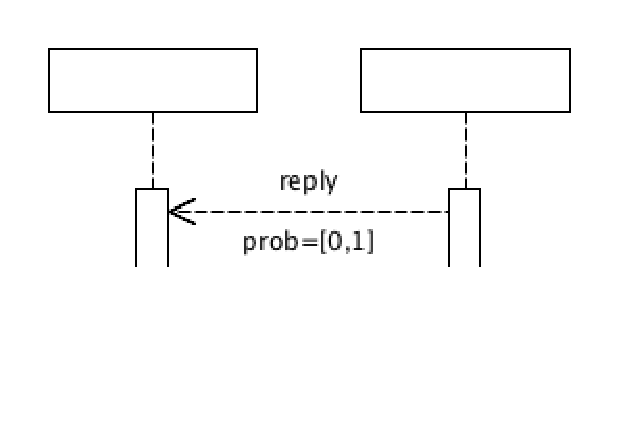
\includegraphics[scale=0.5]{./img/sdReplyMessage}
\input{./img/sdReplyMessage.tex}
\caption{Reply message.}
\label{fig:reply_SD}
\end{subfigure}

\caption{Messages types of a UML sequence diagram.}
\label{fig:messages_SD}
\end{figure}

%%%%%%%%%%%%%%%%%%%%
%\begin{figure}[h!]
%\begin{center}
%\includegraphics[scale=0.5]{./img/sdSyncMessage}
%\end{center}
%\caption{Synchronous message of a UML sequence diagram.}
%\label{fig:sync_SD}
%\end{figure}

From the structural point-of-view the synchronous, assynchronous and reply
messages are equals. They are defined by an interaction between two software
components (a.k.a. \emph{lifelines}) that represents a method
call between them. The message is represented by an arrow with its head varying
as the message type, the method name placed over the arrow and its associated
probability represented by the value assigned to the \texttt{prob} tag. Such value
represents the communication channel's reliability.

\paragraph{Synchronous message: \label{par:syncMessageModeling}} it is described
in a sequence diagram by a solid and closed arrow between two lifelines as shown
by Figure \ref{fig:sync_SD}.  The synchronous message is used to represent a
communication between two components in which the caller halts its execution and
waits for the answer to be provided by the called component. As the caller
component waits for the answer it is necessary having an associated \texttt{reply}
message to each synchronous message used in the model. In the running example,
the \texttt{register} and \texttt{persist} messages represented in
Figure~\ref{fig:oxygenationSituation} are synchronous messages.

%%%%%%%%%%%%%%%%%%%%
%\begin{figure}[h!]
%\begin{center}
%\includegraphics[scale=0.5]{./img/sdAssyncMessage}
%\end{center}
%\caption{Assynchronous message of a UML Sequence Diagram.}
%\label{fig:assync_SD}
%\end{figure}

\paragraph{Assynchronous message: \label{par:assyncMessageModeling}} it is
described by a solid and open arrow between two lifelines, as shown by Figure
\ref{fig:assync_SD}.  The assynchronous message is used to represent a
communication in which the caller sends a signal to the called component but
does not wait for the return. Thus, the assynchronous message does not have an
associated reply message. In the running example, the \texttt{sendSituation}
message represented in Figure~\ref{fig:oxygenationSituation} is an assynchronous message.


%%%%%%%%%%%%%%%%%%%%
%\begin{figure}[h!]
%\begin{center}
%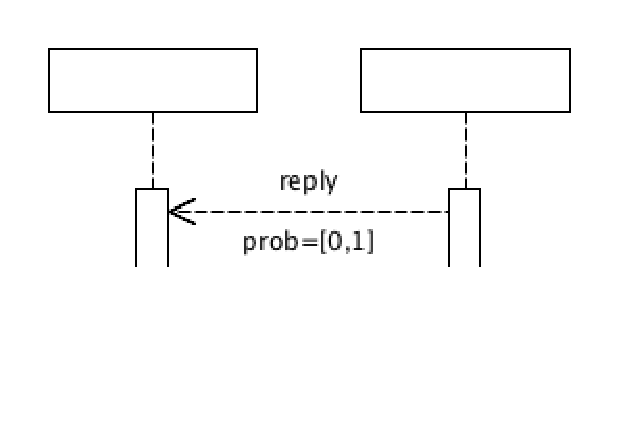
\includegraphics[scale=0.5]{./img/sdReplyMessage}
%\end{center}
%\caption{Reply message of a UML Sequence Diagram.}
%\label{fig:reply_SD}
%\end{figure}

\paragraph{Reply message: \label{par:replyMessageModeling}} it is represented by
a dashed and open arrow directed to the caller lifeline as shown by
Figure~\ref{fig:reply_SD}.  The reply message is used to represent the called
method finished its execution and both control and  result are returned to the caller method.
The name placed over the arrow always starts with \texttt{reply} to
reinforces the message is associated with a synchronous call. In the running
example (c.f. Figure~\ref{fig:oxygenationSituation}) the messages \texttt{replyRegister}, \texttt{replyPersist} and
\texttt{replySendSituation} are examples of reply messages.

%%%%%%%%%%%%%%%%%%%%
\begin{figure}[h!]
\begin{center}
%\includegraphics[scale=0.5]{./img/sdAltFragment}
\resizebox{!}{6cm}{
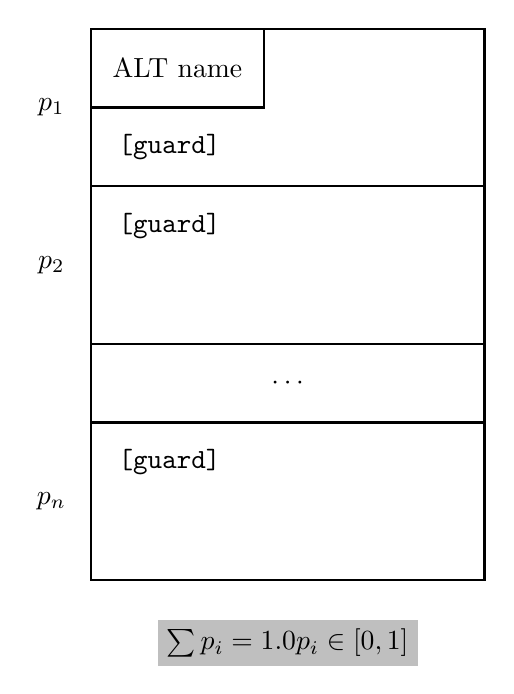
\begin{tikzpicture}[thick]
%%%%%%%%%%%%%%%%%%%%%%%%%%%%%%%%%%%%%%%%%%% HELP LINES
%\draw[help lines] (0,0) grid +(10,10);

%%%%%%%%%%%%%%%%%%%%%%%%%%%%%%%%%%%%%%%%%%% elements
\draw (1,0) rectangle +(5,2);
\node[shape=rectangle, draw=none](p1) at (0.5,6){$p_1$};
\draw (1,2) rectangle +(5,1);
\node[shape=rectangle, draw=none](p2) at (0.5,4){$p_2$};
\draw (1,3) rectangle +(5,2);
\node[shape=rectangle, draw=none](pn) at (0.5,1){$p_n$};
\draw (1,5) rectangle +(5,2);
\node[shape=rectangle, draw=none](ellipsis) at (3.5,2.5){$\cdots$};

%%%%% guards and constraints
\node[shape=rectangle, draw=black, minimum height=1cm, minimum width=2.2cm](alt)at(2.1,6.5){ALT name};
\node[shape=rectangle, draw=none](guard1) at (2,5.5) {\texttt{[guard]}};
\node[shape=rectangle, draw=none](guard2) at (2,4.5) {\texttt{[guard]}};
\node[shape=rectangle, draw=none](guard3) at (2,1.5) {\texttt{[guard]}};
\node[shape=rectangle, fill=gray!50, draw=none](constraint) at (3.5,-0.8) {$\sum p_{i}=1.0$ \\ $p_{i} \in [0,1]$};
\end{tikzpicture}

}
\end{center}
\caption{Alternative fragment of a UML sequence diagram.}
\label{fig:altFrag_SD}
\end{figure}

\paragraph{Alternative fragment:\label{par:altFragModeling}} it is represented
by a rectangle with the \texttt{ALT} tag placed at the top left corner, in
addition to various inner rectangles called \emph{lanes} as shown by
Figure~\ref{fig:altFrag_SD}.  The alternative fragment is used to represent
runtime behavioral variability whose decision is taken based on the runtime
software's context.  Each lane comprises several sequence diagram's elements
defining its associated behavior, which is guarded by a propositional condition
placed inside square brackets. Each lane's guard condition is verified at
runtime and, in case it is satisfied, its comprised behavior is executed.
Although the lanes' guard condition is only verified during runtime due its
dependency to the software's context, the domain especialist defines \emph{a
priori} the execution probability for each lane. Therefore, each lane has an
associated $p_i, 1 \leq i \leq n$ tag whose value represents its execution probability such
the sum of all lane's probability must be equals to $1.0$. 


%%%%%%%%%%%%%%%%%%%%
\begin{figure}[h!]
\begin{center}
%\includegraphics[scale=0.5]{./img/sdLoopFragment}
\resizebox{!}{5cm}{
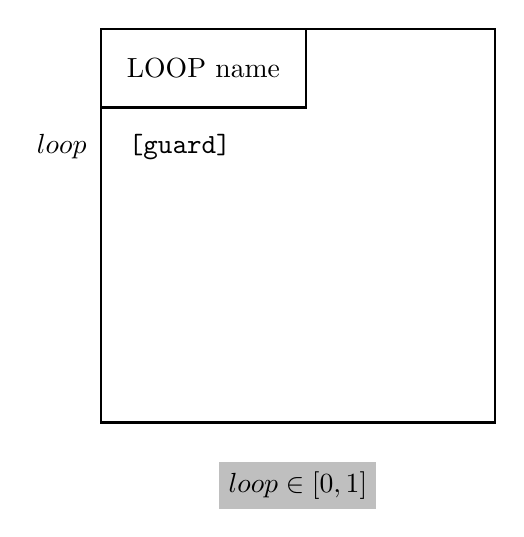
\begin{tikzpicture}[thick]
%%%%%%%%%%%%%%%%%%%%%%%%%%%%%%%%%%%%%%%%%%% HELP LINES
%\draw[help lines] (0,0) grid +(10,10);

%%%%%%%%%%%%%%%%%%%%%%%%%%%%%%%%%%%%%%%%%%% elements
\draw (1,0) rectangle +(5,5);
\node[shape=rectangle, draw=none](p1) at (0.5,3.5){$loop$};
%\draw (1,2) rectangle +(5,1);
%\draw (1,3) rectangle +(5,2);
%\draw (1,5) rectangle +(5,2);


%%%%% guards and constraints
\node[shape=rectangle, draw=black, minimum height=1cm, minimum width=2.6cm](alt)at(2.3,4.5){LOOP name};
\node[shape=rectangle, draw=none](guard) at (2,3.5) {\texttt{[guard]}};
\node[shape=rectangle, fill=gray!50, draw=none](constraint) at (3.5,-0.8) {$loop \in [0,1]$};
\end{tikzpicture}

}
\end{center}
\caption{Loop fragment of a UML sequence diagram.}
\label{fig:loopFrag_SD}
\end{figure}

\paragraph{Loop fragment:\label{par:loopFragModeling}} it is represented by the
rectangle shown by Figure~\ref{fig:loopFrag_SD} with the \texttt{LOOP} tag
placed at the top-left corner and the behavior depicted in its inside. The loop
fragment is used to represent some behavior that repeats a given number of
times. The number of iterations depends on the runtime evaluation of the fragment's
guard condition that is represented by the propositional statement placed inside
the square brackets. Similar to the alternative fragment, the domain expert
must define its execution probability by assigning a
value to the $loop$ tag. Obviously, the probability of not executing the loop
fragment assumes the complement of $1-loop$. 

%%%%%%%%%%%%%%%%%%%%
\begin{figure}[h!]
\begin{center}
%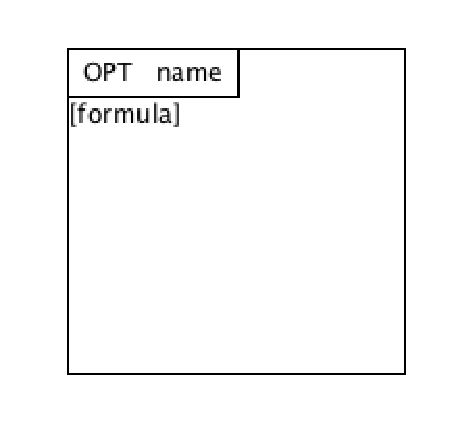
\includegraphics[scale=0.5]{./img/sdOptFragment}
\resizebox{!}{4.5cm}{
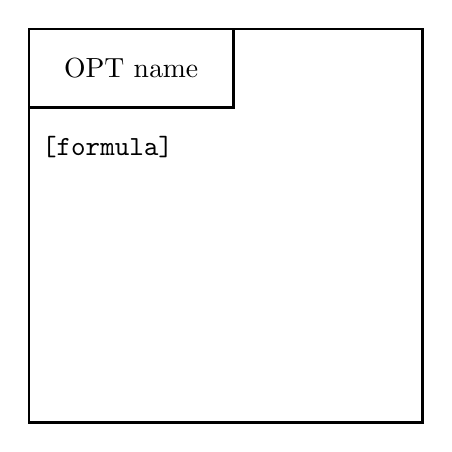
\begin{tikzpicture}[thick]
%%%%%%%%%%%%%%%%%%%%%%%%%%%%%%%%%%%%%%%%%%% HELP LINES
%\draw[help lines] (0,0) grid +(10,10);

%%%%%%%%%%%%%%%%%%%%%%%%%%%%%%%%%%%%%%%%%%% elements
\draw (1,0) rectangle +(5,5);

%%%%% guards and constraints
\node[shape=rectangle, draw=black, minimum height=1cm, minimum width=2.6cm](alt)at(2.3,4.5){OPT name};
\node[shape=rectangle, draw=none](guard) at (2,3.5) {\texttt{[formula]}};
\end{tikzpicture}


}
\end{center}
\caption{Optional fragment of a UML sequence diagram.}
\label{fig:optFrag_SD}
\end{figure}

\paragraph{Optional fragment:\label{par:optFragModeling}} it is represented by
a rectangle containing the tag \texttt{OPT} at its top-left corner followed by
its name, as depicted by Figure \ref{fig:optFrag_SD}. In its original
semantics, it represents the behavioral variability that occurs in runtime,
e.g., it can be used to model the behavior of an \texttt{if} conditional
statement. However, such element plays a major role in the context of modeling
the behavioral variability of software product lines since such variability can happens in
different times -- not only during runtime). The optional fragment is the
element responsible to represent, in an uniform manner, \emph{all} the possible
behavioral variability of a software product line because it relates the
fragment's behavior to the  presence or absence of features in a set of
configurations.  The behavior is defined by the UML sequence diagram's elements
comprised inside the fragment and the guard condition is expressed by a
propositional formula inside square brackets whose atoms are named as the
feature's names.  Such formula indeed represents the \emph{presence condition}
that must be fulfilled by configurations so that they execute  its represented
behavior.  Thus, in a brief, such element had its semantic changed in this work
in order to (a) represent all kinds of variability by (b) enclosing the
variable behavior in optional fragments (c) whose guard's formula will denote
the set of partial configurations for which it will be considered. The
configurations that do not comprise its satisfiability set will not present its
behavior. 
%Thus, in  general, the satisfiability set computed for the guard
%condition formula results into the set of partial configurations which will
%comprise and execute the fragment's behavior.

In the case of the running example the sequence diagrams shown by
figures~\ref{fig:oxygenationSituation} and \ref{fig:temperatureSituation}
represents behavioral variability points related to the activity ``System
identifies \underline{situation}''. In Figure~\ref{fig:oxygenationSituation}
the outermost optional fragment is associated to the optional
\emph{Oxygenation} feature (cf. Figure~\ref{fig:fm}) since its guard condition
is the atom \texttt{Oxygenation}. By your turn, such optional fragment also has
two variability points related to data persistence. The first fragment is
associated to the \emph{SQLite} feature by the atom \texttt{SQLite} and the
second fragment is associated to the \emph{Memory} feature by the atom
\texttt{Memory}. Note that both $SQLite$ and $Memory$ are alternative features,
but they are represented uniformly by optional combined fragments. As the
behavior of the \emph{Temperature} feature is similar to the behavior of
\emph{Oxygenation} feature, the rationale above also applies to the sequence
diagram depicted by Figure~\ref{fig:temperatureSituation}.

\vspace{1cm}

In summary, the UML activity and sequence diagrams can be used to represent the
behavioral characteristics of a software product line. On the one hand, activity
diagrams are used to represent the major tasks and execution flows that all
instantied products must perform. On the other hand, sequence diagrams represent
the shared and variable behavior, such a sequence diagram is a behavioral
detailing of an activity. Both diagrams are enriched with the UML MARTE profile
in order to allow them representing probabilistic behavioral information.

\begin{figure}[h!]
\centering
\begin{tikzpicture}[baseline, level 1/.style={sibling distance=50mm}]
\node[rectangle, draw=black](BF){Behavioral Fragment}
  child[open triangle 45-, thick]{node[rectangle, draw=black](AD){Activity\\ Diagram}}
  child[open triangle 45-,, thick]{node[rectangle, draw=black](SD){Sequence\\ Diagram}}
  child[open triangle 45-,, thick]{node[rectangle, draw=black](OCF){Optional \\combined fragment}};
  
  \draw [-latex, thick](AD) -- node[below, near end, draw=none]{} (SD);
  \draw [-diamond](OCF.north) |- +(2.3cm,0.5cm) |- (OCF.east);
  \draw [diamond-](SD) -- (OCF);
\end{tikzpicture}
\caption{Associations between Behavioral Fragments, Sequence diagrams and Optional combined fragments}
\label{fig:nestedBehavioral}
\end{figure}

Finally, it worths describing the relationship among the UML behavioral
diagrams considered in this work. Such relations are represented by
Figure~\ref{fig:nestedBehavioral}. Any kind of
behavioral representation is considered a \emph{behavioral fragment} which can be
specialized into an activity diagram, sequence diagram or an optional combined
fragment. The association from activity diagram and sequence diagram represents
the refinement relation between an activity and its associated sequence diagram.
In addition, a sequence diagram can be comprised of several optional combined fragments
for representing its behavioral variability. By your turn, an optional combined
fragment has its behavior represented by a sequence diagram which, by your turn,
can have variability points described by other optional combined fragments. Such
relations are important for the evaluation method due the steps of the
evaluation method considers and explores the polymorphism between such elements
when evaluating the reliability of each behavioral fragment. 








%%%%%%%%%%%%%%%%%%%%%%%%%%%%%%%%%%%%%%%%%%%%%%%%%%%%%%%%%%%%%%%%%%%%%%%%%%%%%%%%
%% RELIABILITY OF UML BEHAVIORAL MODELS
%%%%%%%%%%%%%%%%%%%%%%%%%%%%%%%%%%%%%%%%%%%%%%%%%%%%%%%%%%%%%%%%%%%%%%%%%%%%%%%%
\section{Reliability of UML Behavioral Models.
	\label{sec:reliabilityUMLBehavioralModels}}

%As presented previously, it is possible to represent the whole software product
%line's behavior using most of the UML activity and sequence diagrams' elements
%as they are defined. The only exception is the Optional Combined Fragment whose
%semantics is adapted to address the behavioral variability inherent of software
%product lines. Both UML Activity and Sequence diagrams can be transformed into
%probabilistic models enriched with variability (ie. FDTMCs) by employing the
%transformation rules defined for their behavioral elements.  Although there are
%well-known methods\cite{Ghezzi, Genaina} for computing reliability based on the
%FDTMCs resulting from transformation operations, the reliability notion on UML
%behavioral diagrams is still not defined.

Intuitively, the software reliability computed from a UML behavioral diagram is
the execution probability of all its possible behaviors from the first until
last element, such the software behavior is defined by a set of execution
sequences of actions or methods (a.k.a. \emph{paths}). Thus the reliability
analysis implies into identifying and computing the probabilities of all
possible executions represented in the diagram. Since each possible execution
in a behavioral diagram is a sequence of UML behavioral elements, the
probability associated to each element placed along the path must be considered
when computing its probability. 

A path in a behavioral diagram consists of a finite sequence of behavioral
elements such that one element is only executed just after its previous element
finishes its execution. The order which such elements are disposed is temporal
and defined according to the execution manner of the behavioral diagram.
Formally, an execution  path is a partial order defined as: \begin{equation}
	\label{eq:pathDefinition} \varrho = e_1 \alpha_1 e_2 \alpha_2 \ldots
	\alpha_m e_n \end{equation} where $\varrho$ is the execution path;
$e_i, 1 \leq i \leq n$ is each behavioral element comprising the path $\varrho$
and $\alpha_j, 1 \leq j \leq m$ is an action linking two behavioral elements.
Since a path is a \emph{serial} execution of behavioral elements its
reliability is computed as the product of all  elements's reliabilities. An
element in a given place along the path has its \emph{accumulated reliability}
that is computed by multiplying the element's probability and the accumulated
reliability of its next element. Formally, the accumulated reliability of an
element $e$ is given by the recursive function \begin{equation}
	R(e_i)=prob(e_i) \times R(e_i+1)
	\label{eq:accumulatedReliability}\end{equation} where $prob(e_i)$ is
the probability associated to $e_i$ and $R(e_{i+1})$ is the accumulated
reliability computed for its direct sucessor. Thus, considering the accumulated
reliability is computed in a recursive fashion, the path's reliability is given
by the accumulated reliability of its first element, which is defined as:
\begin{equation} \label{eq:pathReliabilityDefinition} R(\varrho) =
	R(e_1)\end{equation} where $R(\varrho)$ is the reliability of the path
$\varrho$ and $R(e_1)$ is the accumulated reliability of the first path's
element. However, the reliability definitio varies according to the semantics
of each behavioral element so that the reliabilities definitions of all
behavioral elements considered in this work are shown in sections
\ref{sec:reliabilityOfActivityDiagramModels} and
\ref{sec:reliabilityOfSequenceDiagramModels}.

Finally, given the relations of behavioral fragments represented by
Figure~\ref{fig:nestedBehavioral} a general definition for the
reliability computation of a behavioral fragment must be useful to
compute the reliability of activity diagram, sequence diagram and optional
combined fragment in an uniform way. According to 
sections \ref{subsec:umlActivityDiagrams} and \ref{subsec:umlSequenceDiagrams},
both activity and sequence diagrams have an unique starting point (the start
node and the first behavioral element, respectively). Thus, given that paths in
activity and sequence diagrams are sequences of behavioral elements (cf.
Definition~\ref{eq:pathDefinition}) and an optional combined fragment comprises
a sequence diagram in its inside, indeed the reliability definition for a
behavioral fragment can be generalized and formally defined as \begin{align}
	R(bf) &= R(\varrho) \nonumber \\
              &= R(e_1) \label{eq:behavioralFragmentReliability} \end{align} where $\varrho$ is the path whose
first element is the unique starting element of the behavioral fragment $bf$. 

%Finally, as an activity diagram is defined based on a finite set of activity
%diagram elements the activity diagram's behavior consists of a finite set of
%paths. Such assumption is particularly valid for activity diagrams containing
%loops in its structure, ie., when an element is linked to previous element, as a
%path is always comprised by a finite sequence of elements. Therefore, to compute
%the activity diagram's reliability, all paths' reliabilities must be considered.
%Given a path execution is independent from any other path's execution, the
%reliability is given by the sum of all paths' reliabilities. It can be defined
%as \begin{equation} \label{eq:splReliabilityDefinition}R(SPL.ad) = R(P) =
%	\sum_{i=1}^{k}{R(\varrho_i)}\end{equation} where $P = \{\varrho_i | 1
%\leq i \leq k\}$ is the set of execution paths of the activity diagram.

% By your turn, given an activity or sequence diagram, its reliability can be
% computed by the sum of the accumulated probabilities of all paths from the
% execution of the first element until the execution end of the last element. As
% path is a sequence of behavioral elements used in behavioral model, to create a
% path from a behavioral element it is necessary obtain its directed sucessors,
% i.e., the elements reachable from the current element in one step. Thus, an
% auxiliary function named \texttt{next()} is defined for both activity and
% sequence diagrams, so from a given behavioral element it returns its directly
% sucessors.
% 
% The \texttt{next()} function varies according to the UML behavioral diagram
% under evaluation. In an activity diagram all elements are linked by transitions
% which allows operate over its elements similar to graphs. Thus, an activity
% diagram can be formally defiend as: \[ AD = (E, T, \rightarrow, I) \] where $E$
% is a set of activity diagram elements, $T$ is a set of transitions, and
% $\rightarrow \in \{E \times T \times E\}$ is the transition relation between
% activity diagram elements.  Given an activity diagram element, its set of
% sucessor elements given by the \texttt{next()} function is the set of elements
% reachable by a single transition, i.e., the set of elements having an incoming
% edge from the current element. Formally, such function can be defined as:
% 
% \[
% 	next(e, \alpha) = \{e' \in E | e \xrightarrow[]{\alpha} e'\}
% \]
% \[
% 	next(e) = \bigcup_{\alpha \in T} next (e, \alpha)
% \]
% The reliability evaluation of a sequence diagram is similar to the execution of
% an activity diagram as the execution order imposed to the comprised elements
% must be considered. However sequence diagrams
% do not establish a direct association between its elements like activity
% diagrams represent by edges. The only relation between the sequence diagram
% elements is the temporal order which they are defined. Thus, instead of
% considering a sequence diagram as a graph it can be considered as a
% partial-ordering of the elements which comprise it. In this case, the
% \texttt{next} function defined for a sequence diagram returns the set of
% elements immediatly after the element under evaluation. Such function may be
% formally defined as:
% 
% \textbf{\textit{Formal definition of nextSD()}}

Therefore the reliability of a behavioral model is computed in an inductive fashion based on
the structure of the UML behavioral model. Considering the software product
line's behavior is expressed by a set of UML behavioral models, its reliability
is given by each behavioral model's reliability and the way such models are
related. On the one hand the reliability of the whole software product line is
defined by the manner how the activities are related in an activity diagram and
how each activity is detailed by a sequence diagram. At the other hand, since
an activity is detailed by its associated sequence diagram its reliability is
also associated to the reliability computed for its sequence diagram. Such
reliabilities notions are explained in details next.


\subsection{Reliability of software product line
	\label{sec:reliabilityOfSoftwareProductLinesAtUmlBehavioralModels}}


To compute the reliability of a software product line it is necessary to
consider the reliabilities of all behavioral diagrams and  the manner how such
diagrams are related. By associating a sequence diagram to each activity it is possible to define the set of all
behavioral diagrams as well as how such sequence diagrams are related.  Thereby,
the reliability of a whole software product line is the reliability of its UML
activity diagram, which can be formally defined as \begin{equation}
	\label{eq:splReliability} R(SPL) = R(SPL.ad) \end{equation} where $SPL$
is the software product line subject of the evaluation and $SPL.ad$ is the
activity diagram representing the  coarse-grained behavior of the $SPL$.

%%%%%%%%%%%%%%%%%%%%
\subsection{Reliability of activity diagram elements
	\label{sec:reliabilityOfActivityDiagramModels}}

According to Definition \ref{eq:splReliability}, the software product line's
reliability is computed based on its activity diagram, which by Definition
\ref{eq:behavioralFragmentReliability}, it is the accumulated reliability of its
first element (i.e. the product of all elements' reliabilities along
the path). Since the reliability function $R$ is inductive in the structure of
the behavioral model it is necessary to compute the accumulated reliability for
each element along the path which is given by the element's probability value multiplied by the
accumulated reliability of its immediately sucessor. Next, the
accumulated reliability definition for each activity diagram's element is
presented. From now on it is meant by behavior any interaction between software components.

\paragraph{Initial node:}
since the initial node does not have an associated behavior its impact over the
reliability computation is null. Thus, its accumulated reliability is equal to
$1.0$ multiplied by the accumulated reliability of its remaining path. Formally
it is defined as \begin{equation} \label{eq:initialNodeReliability}R(in) = 1.0
	\times R\big(next(in)\big)\end{equation} where $in$ is the initial node and
$next(in)$ is the singleton set of its immediately sucessor and $R(next(in))$ is the accumulated probability of such element.

%%%%%%%%%%%%%%%%%%%%
\paragraph{Activity:}
due an activity is detailed by a sequence diagram its reliability varies 
according to such diagram's behavior and the product instantiated.  Thus, it is
agreed to represent the activity's reliability as a variable named as the
activity with the `r' prefix standing for ``reliability''. Formally it is
defined as \begin{equation}\label{eq:activityReliability}R(a) = rActivity \times
	R\big(next(a)\big)\end{equation} where $a$ is an activity named $Activity$;
$rActivity, rActivity \in [0,1]$ is the variable representing the activity's
reliability, $next(a)$ is the sucessor of $a$ and $R(next(a))$ is the accumulated reliability of its immediately
sucessor.


%%%%%%%%%%%%%%%%%%%%
\paragraph{Decision node:}
the decision node is the element that  splits the behavior into different paths
such each alternative path has an associated execution probability
defined by the domain expert (c.f. Figure~\ref{fig:decision_AD}). Given that each path is independently executed 
from the others, the reliability of the decision node is the sum of the
cummulative reliabilities of all alternative paths. Such reliability
definition is formally given by \begin{equation}
	\label{eq:decisionNodeReliability} R(d) = \sum_{i=1}^{n} pr_{i} \times
	R\big(next(d, i)\big) \end{equation} where $n$ is the number of outgoing edges
of the decision node $d$, $pr_i$ is the
probability associated to the $i^{th}$ edge, $next(d, i)$ is the singleton set
of the immediately sucessor of $d$ by the edge $i$ and $R(next(d,i))$ is the
accumulated probability of such element.


%%%%%%%%%%%%%%%%%%%%
\paragraph{Merge node:}
the merge node joins different behavioral branches into a single path without
any interaction between software components. Thus, its impact over the
reliability computation is null and its accumulated reliability is formally
defined as \begin{equation} \label{eq:mergeNodeReliability} R(m) = 1.0 \times
	R\big(next(m)\big) \end{equation} where $next(m)$ is the immediately sucessor of $m$ and $R(next(m))$ is the accumulated
reliability computed for such element.


%%%%%%%%%%%%%%%%%%%%
\paragraph{End node:}
the end node determines the execution's end of an activity diagram without any
associated behavior such its contribution to the accumulated reliability is null.
It is also the base case of the recursive function $R$ when computing the
reliability of an activity diagram. It is formally defined as \begin{equation}
	\label{eq:endNodeReliability} R(e) = 1.0 \end{equation} where $e$ is the
end node.

%\paragraph{Reliability function for activity diagrams} Given the explanations
%above the function to compute the reliability of an Activity Diagram is a
%recursive function for computing all possible paths from the initial to the
%final elements. As each possible path has an expression associated to it, the
%reliability expression given by the reliability function is a sum of
%expressions, each one representing one possible path. Given that a path is a
%sequence of activity diagram elements, the reliability of a path is given by
%the cummulative reliability of the elements it comprises, i.e., the cummulative
%reliability is given by the product of the reliability of an element and the
%reliability of all possible paths starting from it. Thus, the recursive
%function \texttt{reliability(AD)} to compute the reliability of an activity
%diagram is defined as:
%\textbf{\textit{Insert the algorithm for the reliability function.}}


%%%%%%%%%%%%%%%%%%%%%%%%%%%%%%%%%%%%%%%%
\subsection{Reliability of sequence diagram models
	\label{sec:reliabilityOfSequenceDiagramModels}}

The reliability computation of a sequence diagram resembles the reliability
computation of models described by activity diagrams.  For both the reliability
is given by the accumulated reliability of the first element (as stated by
Definition~\ref{eq:behavioralFragmentReliability}) and the path's
reliability is inductively computed on the path structure by the product of all
elements in its sequence (as stated by Definition~\ref{eq:accumulatedReliability}). However, the sequence diagram's representation
structure and the need of representing the behavioral variability turn the
reliability function $R$ for sequence diagram slightly different from the
reliability function of activity diagram.

The first difference stems from the representation structure of a sequence diagram: 
differently of activity diagram whose elements are linked by transitions, there is no link between the elements
comprising a sequence diagram. The unique relation
between the sequence diagram's elements is the point where each element is
represented in the diagram which, given its top-down reading way, imposes a
temporal sequence for its elements. Therefore, to compute the accumulated reliability
of a sequence diagram element it is necessary consider which elements may
execute in the next step.

In addition, the sequence diagram is the responsible for representing the
software product line's behavioral variability as some behavioral
fragments will comprise a set of products but will not in another set. Given the
accumulated reliability of an element is a recursive function,
such function must be able to consider such variability of the
software product line in an uniform manner.

Thus the reliability function $R$ for sequence diagrams has to deal
with the temporal link between the elements of a variable behavioral diagram.
Both characteristics impose a semantic change of a sequence diagram element for
representing the inherent variability of a software product line and also
consider the sequence of the sequence diagram elements as a partial-ordering.
The definitions of reliability function $R$ for the sequence diagram's elements are presented next. 



%%%%%%%%%%%%%%%%%%%%
\paragraph{Synchronous, assynchronous and reply messages:
	\label{subsec:relMessages}}
albeit the execution of synchronous, assynchronous and reply messages have
different execution modes (c.f. Section~\ref{subsec:umlSequenceDiagrams}), they are similar from the structural and
reliability points of view: all of them are a communication
between two software components that is accordingly performed  bounded by the
communication channel's reliability. Thus  the
accumulated reliability for such messages is given by the probability associated
to the message multiplied by the accumulated reliability of its next
element. Such definition is formally given by: \begin{equation}
	\label{eq:syncMessageReliability} R(m) = prob(m) \times R\big(next(m)\big)
\end{equation} where $prob(m)$ is the function
that returns the probability value associated to the message $m$, $next(m)$ is the function that returns its next executable element
and $R(next(m))$ is the cummulative reliability computed for the
sucessor of $m$.

%%%%%%%%%%%%%%%%%%%%
%\paragraph{Assynchronous message: \label{subsec:relAssynchronousMessage}} 
%Although the assynchronous message is different from synchronous message since it
%does not have an associated reply message, the semantics of both are equal as
%their reliabilities are computed by multiplying the message's probability and
%its sucessor's cummulative reliability. Thus assynchronous message's reliability
%is given by: \begin{equation} \label{eq:assyncMessageReliability} R(a) = prob(a)
%	\times R(next(a)) \end{equation} where $a$ is the assynchronous message,
%$prob(a)$ is the probability value associated to $a$, $next(a)$ is the function
%that returns the singleton set of the immediately sucessor of $a$, and
%$R(next(a))$ is the cummulative reliability computed for the sucessor of $a$.
%
%
%
%%%%%%%%%%%%%%%%%%%%%
%\paragraph{Reply message: \label{subsec:relReplyMessage}}
%% As a reply message interacts with the component of the caller method it has an
%% associated probability of accomplishing the control return, which is given by
%% the \texttt{prob}. In case the reply message executes accordingly the execution
%% continues from the element just after the reply message.
%The cummulative reliability for a reply message is given by the probability
%associated to the message multiplied by the cummulative reliability of its next
%element. Such reliability is defined as: \begin{equation}
%	\label{eq:replyMessageReliability}R(r) = prob(r) \times R(next(r))
%\end{equation} where $r$ is the reply message, $prob(r)$ is the probability
%value associated to $r$, $next(r)$ is the singleton set of its immediate
%sucessor and $R(next(r))$ is the cummulative reliability computed for the
%sucessor of $r$. 

%%%%%%%%%%%%%%%%%%%%
\paragraph{Loop fragment: \label{subsec:relLoopFragment}}
%The loop fragment is used to represent a behavior that repeats a given number of
%times according to the runtime context.  In practice such execution is the
%sequential execution of the path defined by the loop fragment, such the path
%appears several times in the sequence. 
%Although it is not possible to know how many times a loop fragment will execute
%during modeling time, the domain expert can assign probabilities values for
%executing and not-executing the loop's behavior. 
%Given the sequential execution of a behavioral diagram is characterized by the
%multiplication of the element to next element, if we consider each execution of
%the loop as an element, we will have n-executions of the loop. 
%Thus, the reliability of the loop fragment can be defined as the reliability of
%the loop fragment power to n iterations, multiplied by the reliability of the
%element just after the loop. Thus, it can be defined as being:
Since the loop fragment has a probability value defined by the \texttt{loop} variable for
the cases it is executed (consequently its complement represents the probability
of not executing the loop), such value must be considered for its reliability
definition.  In the case the loop's behavior is executed, its inner content's reliability must also be taken into account, otherwise the non-execution probability must be considered. Such
inner behavior is, indeed, represented by a sequence diagram associated to the
loop fragment. Thus, the reliability of a loop fragment is given by the
accumulated probability of both loop's execution and non-execution. Such
reliability is formally defined as \begin{equation} \label{eq:loopFragmentReliability}
	R(l) = \Big(prob(loop) \times R\big(SD(l)\big) + \big(1-prob(loop)\big)\Big) \times
	R\big(next(l)\big) \end{equation} where $prob(loop)$ is the fragment's
execution probability, $SD(l)$ is the function that returns the sequence diagram
of the loop $l$, $R(SD(l))$ is the reliability computed for such diagram (i.e. the loop's innerbehavior), $1-prob(loop)$ is the probability of not executing $l$, $next(l)$ is the directly sucessor of $l$ and
$R(next(l))$ is the accumulated reliability of the immediately sucessor of $l$.

%%%%%%%%%%%%%%%%%%%%
\paragraph{Alternative fragment: \label{subsec:relAlternativeFragment}} as the
alternative fragment represents the behavior splitting into several
alternatives in practice it creates several possible execution flows from it
such each alternative has its execution probability defined by the domain
expert. Besides, since each alternative's behavior is represented by a sequence
diagram, its reliability is given by the reliability computed for its associated
sequence diagram. Thus, the reliability of each alternative is given by its
choice probability multiplied by the reliability computed for its sequence
diagram. 

Whatever branch taken the path continues from the element just after the
alternative fragment. The cummulative reliability of the alternative fragment
must consider the reliability of the path remaining after it, that is computed
as the cummulative reliability of its drectly sucessor. Thus, the cummulative
reliability of the alternative fragment is formally defined as: \begin{equation}
	\label{eq:altFragmentReliability}R(a) = \Big(\sum pr_{i} \times
	R\big(SD(alt_{i})\big)\Big) \times R\big(next(a)\big) \end{equation} where $pr_{i}$ is the
execution probability associated to the $i^{th}$ alternative, $SD(alt_{i})$ is the
sequence diagram of the $i^{th}$ alternative, $R(SD(alt_i))$ is the reliability
computed for the sequence diagram of the $i^{th}$ alternative and $R(next(a))$ is
the cummulative reliability computed for the sucessor element of the alternative
fragment.

%%%%%%%%%%%%%%%%%%%%
\paragraph{Optional fragment: \label{subsec:relOptionFragment}}
the optional behavioral fragment represents the behavioral variability of
software product lines according to the presence or absence of features in a configuration. 
%When a behavioral fragment is present at a product, the behavior represented by
%its content will be part of the execution path, so its will be considered when
%computing the cummulative reliability for the optional fragment.  Otherwise,
%when a product configuration does not fulfill the guard condition of the
%optional fragment, the cummulative reliability of the optional fragment must no
%affects the cummulative reliability of the sequence diagram where it appears.
An optional fragment will always be considered by the paths passing
through him but it is necessary to define when its reliability must be
considered or not, such it will not impact the computation. The accumulated
reliability for the optional fragment is thus computed based on the fragments'
behavior presence or absence, in addition to the accumulated reliability
computed from its next element. Formally it is defined as: \begin{equation}
	\label{eq:optionalFragmentReliability}R(o) = R\big(SD(o)\big)^{p} \times
	R\big(next(o)\big)\end{equation} where $SD(o)$ is the sequence diagram
associated to the optional combined fragment $o$, $R(SD(o))$ is the reliability
computed for the sequence diagram associated to $o$, $p \in \{0,1\}$ indicates
the fragment presence (1) or absence (0) and $R(next(o))$ is the accumulated 
reliability of the fragment's sucessor. 

In the case of the running example, both sequence diagrams shown by
figures~\ref{fig:oxygenationSituation} and \ref{fig:temperatureSituation} have
their behaviors varying according to $SQLite$ and $Memory$ features due they
are related to the fragments \texttt{SQLite} and \texttt{Memory}, respectively.
In addition both features are alternative according to the feature model
represented in Figure~\ref{fig:fm}. Thus, whenever one of the persistence
features is present in a configuration the other one is necessarily absent such
its behavior must not affect the reliability computation. In the case of $SQLite$
is part of the configuration the $p$ exponent in its term assumes 1, meanwhile
the $p$ exponent of the term related to $Memory$ feature assumes 0 to represent
its absence. Thus, the reliability of the \texttt{SQLite} fragment is given by
\begin{align}
	R(SQLite)=& R\big(SD(\mathtt{SQLite})\big)^1 \times R\big(next(\mathtt{SQLite})\big) \nonumber \\
	& R\big(SD(\mathtt{SQLite})\big) \times R\big(SD(\mathtt{Memory})\big)^0 \times R\big(\ next(\mathtt{Memory}) \big) \nonumber \\
	& R\big(SD(\mathtt{SQLite})\big) \times 1 \times R\big(\ next(\mathtt{Memory}) \big) \nonumber
\end{align} which, indeed, only considers the reliability of the fragment
associated to $SQLite$ feature. Conversely, the same rationale holds for the cases where
\emph{Memory} is present and \emph{SQLite} is absent in the configuration. 








%%%%%%%%%%%%%%%%%%%%%%%%%%%%%%%%%%%%%%%%%%%%%%%%%%%%%%%%%%%%%%%%%%%%%%%%%%%%%%%%
%% TRANSFORMATION FROM UML TO FDTMC
%%%%%%%%%%%%%%%%%%%%%%%%%%%%%%%%%%%%%%%%%%%%%%%%%%%%%%%%%%%%%%%%%%%%%%%%%%%%%%%%
\section{Transformation from UML to FDTMC \label{sec:transformationUMLFDTMC}}

Once the whole behavior of a software product line is represented by a set of
UML behavioral diagrams it can be transformed into fully probabilistic models
that later will be subject to reliability analysis. However, given the
expressiveness of UML behavioral diagrams (messages execution modes in addition
to alternative, iterable and optional behaviors) such characteristics must also
be considered by the probabilistic models. In this context, the FDTMC is a
suitable modeling notation as it is able to represent the variable and
probabilistic behavior of a software product line.

The UML behavioral models present an \emph{action-based} view of the software
product line's behavior due they represent how the variable behavior is defined
by the behavioral elements and executed by the software components. Meanwhile,
FDTMC provides the corresponding \emph{state-based} view since it represents the
behavioral characteristics by expressing how the software product line's states
vary as long as its behavior is executed. In an FDTMC, each state represents the
observable characteristics reached by the software after executing its
respective UML element. 

Given the dependency between the action-based and state-based views, a
translation rule to an FDTMC sub-structure is defined for each UML behavioral element. A
transformation rule is defined by two parts: the left-hand side shows the
UML element being transformed and the right-hand side shows its resulting FDTMC
sub-structure. From now on it is agreed that elements depicted by solid lines at
the right-hand side are the FDTMC's states or edges newly created by the
transformation rule, while the elements represented in dashed lines were already
existing. It is also agreed naming \emph{current state} the state from which the
FDTMC substructure will be build. Thereby, a whole UML behavioral model can be
translated into its respective FDTMC by applying the transformation rule of each
behavioral element in a stepwise fashion. Next the translation rule and the
resulting FDTMC for each UML behavioral element is presented jointly with the
description of its state-based view.

%%%%%%%%%%%%%%%%%%%%%%%%%%%%%%%%%%%%%%%%
%% Transformation Rules for Activity Diagram Elements
%%%%%%%%%%%%%%%%%%%%%%%%%%%%%%%%%%%%%%%%
\subsection{Transformation Rules for Activity Diagram Elements
	\label{subsec:transfomrationRulesActivityDiagramElements}}










%%%%%%%%%%%%%%%%%%%%
\begin{figure}[h!]
\begin{center}
\begin{tikzpicture}
	\centering
	%\begin{tikzpicture}
% \draw[help lines] (0,0) grid +(3, 1);
% \draw[help lines] (0,0) grid +(3,-1);
\node[adStart](start){};
\node[initial, thick](initial) at (3,0){(\textit{init})};
\node[thick](regular) at (5,0){};
\node[error,thick](error) at (5,-2){(\textit{error})};
\draw[thick, dashed](1,1) -- (1,-2);
\draw[thick, ->, line width=1pt] (1.5,0) -- (initial.west);
\draw[thick, ->, line width=1pt] (initial.east) -- node[draw=none, rectangle, above]{$1.0$}(regular.west);
\draw[thick, ->, line width=1pt] (initial.south) |- node[draw=none, rectangle, auto]{$0.0$}(error.west);
%\end{tikzpicture}

\end{tikzpicture}
%\includegraphics[scale=0.5]{./img/adTransInitNode}
\end{center}
\caption{Transformation rule for an initial node of an activity diagram.}
\label{fig:transInit_AD}
\end{figure}

\paragraph{Initial node: \label{par:initialNodeTransformation}}
the 
resulting FDTMC shown by Figure~\ref{fig:transInit_AD} is comprised of three
states and two edges. The labeled states \texttt{init} and \texttt{error} represent,
respectively,  the state where the execution begins and the state
representing some error occurred during the diagram execution. The edge from
\texttt{init} to the unlabeled state has the  associated probability
value $1.0$ and, due the basic FDTMC's property, its complement edge has $0.0$ as
probability value. 

The state-based view provided by the resulting FDTMC means the execution starts
(\texttt{init} state) and proceeds with probability equals to $1.0$ to the next
state. Such value follows from the fact there is no software behavior associated
to the initial node, so its failure probability is equal to $0.0$. 

%%%%%%%%%%%%%%%%%%%%
\begin{figure}[h!]
\begin{center}
\begin{tikzpicture} 
	\centering
	%\begin{tikzpicture}[scale=0.6]
%%%%%%%%%%%%%%%%%%% HELP LINES
% \draw[help lines] (0,0) grid +(6,1);
% \draw[help lines] (0,0) grid +(6,-1);
%%%%%%%%%%%%%%%%%%% NODES
\node[fill=none, draw=none](transp1) at (-1.5,0){$\dots$};
\node[adActiv](activity) at (0.5,0) {Activity};
\node[fill=none, draw=none](transp2) at (2.5,0){$\dots$};

\node[circle, dashed](current) at (4, 1) {};
\node[circle](next) at (6, 1) {};
\node[error, circle, dashed](error) at (6,-1) {(\textit{error})};

\node[rectangle, draw=none, fill=gray!50](constraint) at (5,-2.5){$rActivity \in [0,1]$};

\draw[thick, dashed](3,1) -- (3,-1);
\draw[thick,->, line width=1pt](transp1.east) -- (activity.west);
\draw[thick,->, line width=1pt](activity.east) -- (transp2.west);
\draw[thick,->, line width=1pt](current.east) -- node[midway, yshift=0.3cm, fill=none, draw=none]{rActivity} (next.west);
\draw[thick,->, line width=1pt](current.south) |- node[midway, yshift=-0.3cm, fill=none, draw=none]{1-rActivity}(error.west);

%\end{tikzpicture}
 
\end{tikzpicture}
%\includegraphics[scale=0.5]{./img/adTransActivity}
\end{center}
\caption{Transformation rule for an activity node of an activity diagram.}
\label{fig:transActiv_AD}
\end{figure}

\paragraph{Activity: \label{par:activityTransformation}} 
intuitively, the reliability of an
activity is the reliability computed by its associated sequence diagram.
The activity's transformation rule represented by
Figure~\ref{fig:transActiv_AD} comprises a new state and two new edges. The
edge directed from the current to the newly created state has its probability
represented by the \textit{rActivity} variable, $rActivity \in [0,1]$, whereas the edge directed to the
error state assumes its complement $(1-rActivity)$.

The current state represents the moment just before the activity execution. With
a probability equals to the value assumed by \emph{rActivity}, its associated
behavior is performed without errors and such condition is represented by the
newly created state. Following the naming convention adopted by the UML behavioral modeling (c.f. Section~\ref{subsec:umlActivityDiagrams}) the edge's parameter is named as the activity's name
with the prefix `r' standing out for ``reliability''. In case of an error
occurred anywhere of the sequence diagram associated to the activity, such
condition is represented by the error state that is reached with the probability
given by $1-rActivity$. 


%%%%%%%%%%%%%%%%%%%%
\begin{figure}[h!]
\begin{center}
\begin{tikzpicture}
    %%%%%%%%%%%%%%%%%%% HELP LINES
% \draw[help lines] (0,0) grid + (6,1);
% \draw[help lines] (0,0) grid + (6,-1);
%%%%%%%%%%%%%%%%%%% NODES
\node[fill=none, draw=none](init) at(-0.5,0) {$\dots$};
\node[adDecis](decision)at(1,0) {};
\node[transpNode](dec1) at(2,1) {};
\node[transpNode](dec2) at(2,-1){};
\node[transpNode](decM) at(1.5, 0){$\dots$};

\node[transpNode](befDec) at (3,0){};
\node[circle, dashed](fdecision) at (4,0) {};
\node[circle](fdec1) at (5,1) {};
\node[transpNode](fdecm) at (5,0) {$\dots$};
\node[circle](fdec2) at (5,-1) {};

\node[fill=none, draw=none, rectangle, fill=gray!50](constraint) at (4.5,-1.7){$\sum p_i = 1.0$};
%%%%%%%%%%%%%%%%%%% EDGES
\draw[thick, line width=1pt, ->] (init) -- (decision);
\draw[thick, line width=1pt, ->] (decision) -- node[fill=none, draw=none, xshift=-0.2cm, yshift=0.2cm]{$p_1$}(dec1);
\draw[thick, line width=1pt, ->] (decision) -- node[fill=none, draw=none, xshift=-0.2cm, yshift=-0.2cm]{$p_n$}(dec2);
\draw[thick, dashed] (3,1) -- (3,-1);
\draw[thick, line width=1pt, ->] (befDec) -- (fdecision);
\draw[thick, line width=1pt, ->] (fdecision) -- node[fill=none, draw=none, xshift=-0.2cm, yshift=0.2cm]{$p_1$}(fdec1);
\draw[thick, line width=1pt, ->] (fdecision) -- node[fill=none, draw=none, xshift=-0.2cm, yshift=-0.2cm]{$p_n$}(fdec2);

    \end{tikzpicture}
%\includegraphics[scale=0.5]{./img/adTransDecisNode}
\end{center}
\caption{Transformation rule for a decision node of an activity diagram.}
\label{fig:transDecis_AD}
\end{figure}

\paragraph{Decision node: \label{par:decisionNodeTransformation}}
the translation rule shown by Figure \ref{fig:transDecis_AD} results
into an FDTMC comprised of as many newly edges and states leaving the FDTMC's
current state as the alternatives of the decision node. 

The state-based view provided by the FDTMC means the software execution may
proceed from the current state to the first state of each alternative with the
probability associated to its respective edge. The current state represents the
software state just before the decision is taken and each newly created state
represents the software state just before its behavioral branch starts its
execution. As each decision of a decision node has a probability value assigned
by the domain expert, such probabilities are considered when creating each edge
leaving the current state of the FDTMC. Given the basic property of FDTMCs the
probabilities of all edges leaving the current state must sum $1.0$. Finally,
as there is no software behavior associated to the UML decision node, there is
no edge from current to the \texttt{error} state. 

%%%%%%%%%%%%%%%%%%%%
\begin{figure}[h!]
\begin{center}
\begin{tikzpicture}
    \centering
    %%%%%%%%%%%%%%%%%%% HELP LINES
% \draw[help lines] (0,0) grid +(6,1);
% \draw[help lines] (0,0) grid +(6,-1);
%%%%%%%%%%%%%%%%%%% NODES
\node[transpNode](act1) at (0,1){};
\node[transpNode](actM) at (0,0){};
\node[transpNode](act2) at (0,-1){};
\node[adMerge](merge) at (1,0){};
\node[transpNode](act3) at (2,0){};

\node[circle, dashed](fAct1) at (3, 1){};
\node[circle, dashed](fActM) at (3, 0){};
\node[circle, dashed](fAct2) at (3,-1){};
\node[circle](fMerge) at (4.5,0){};
\node[circle](fAct3) at (6,0){};
%%%%%%%%%%%%%%%%%%% EDGES
\draw[thick, line width=1pt, ->] (act1) -- (merge);
\draw[thick, line width=1pt, ->] (actM) -- (merge);
\draw[thick, line width=1pt, ->] (act2) -- (merge);
\draw[thick, line width=1pt, ->] (merge) -- (act3);

\draw[thick, line width=1pt, dashed] (2.5,1) -- (2.5,-1);

\draw[thick, line width=1pt, ->](fAct1) --node[draw=none, fill=none, midway, yshift=0.2cm]{\scriptsize $1.0$}(fMerge);
\draw[thick, line width=1pt, ->](fActM) --node[draw=none, fill=none, midway, yshift=0.2cm]{\scriptsize $1.0$}(fMerge);
\draw[thick, line width=1pt, ->](fAct2) --node[draw=none, fill=none, midway, yshift=0.2cm]{\scriptsize $1.0$}(fMerge);
\draw[thick, line width=1pt, ->](fMerge) -- node[draw=none, fill=none, midway, yshift=0.2cm]{$1.0$}(fAct3);

\end{tikzpicture}
%\includegraphics[scale=0.5]{./img/adTransMergeNode}
\end{center}
\caption{Transformation rule for a merge node of an activity diagram.}
\label{fig:transMerge_AD}
\end{figure}

\paragraph{Merge node: \label{par:mergeNodeTransformation}} 
the resulting FDTMC shown by Figure~\ref{fig:transMerge_AD} is comprised of
several newly created elements namely: two states, an edge between both states
with probability equals to $1.0$ and as many edges as the number of existing
states to be merged. Such edges also have $1.0$ as transition's probability. 

The FDTMC's state-based view represents by each current state the execution's
end of an alternative behavioral branch while the first newly created state
represents the merging state, ie., the software's state where all alternatives
are ready to merge. From the merging state, the execution proceeds to the merged
state (the second state created by the transformation rule) with probability
equal to $1.0$, due there is no software components interaction enrolled in this
task.

%From the merging state the execution proceeds to the merged state (the second
%state created by the transformation rule) with an probability equals to $1.0$.
%The merged state indicates the execution may proceed from it by a single
%execution flow. As there is no software behavior associated to the alternatives
%merging, the transition from merging to merged states has probability equals to
%$1.0$.

%%%%%%%%%%%%%%%%%%%%
\begin{figure}[h!]
\begin{center}
\begin{tikzpicture}
    \centering
    %%%%%%%%%%%%%%%%%%% HELP LINES
% \draw[help lines] (0,0) grid +(2,1);
% \draw[help lines] (0,0) grid +(2,-1);
%%%%%%%%%%%%%%%%%%% NODES
\node [adStart]at (0,0){}; \node[circle, minimum width=9mm, text width=0, thick, draw=black](end) at (0,0){};
\node [success, circle, dashed](success) at (2.5,0) {(\textit{success})};
%%%%%%%%%%%%%%%%%%% EDGES
\draw[thick, dashed, line width=1pt] (1,1) -- (1,-1);
\path[->] (success) edge [loop right, line width=1pt] node [draw=none]{$1.0$}();

\end{tikzpicture}
%\includegraphics[scale=0.5]{./img/adTransEndNode}
\end{center}
\caption{Transformation rule for an end node of an activity diagram.}
\label{fig:transEnd_AD}
\end{figure}

\paragraph{End node: \label{par:endNodeTransformation}} 
the transformation rule shown by Figure~\ref{fig:transEnd_AD} results into an
FDTMC comprised of a newly created self-edge with probability equals to $1.0$ and
a new label placed at the current state. 

The state-based view of the resulting FDTMC represents the activity diagram
execution has ended successfully due the execution has reached the final
``\emph{success}'' labeled state. As the success state has no associated
components interaction the self-edge assumes the $1.0$ probability value that
transforms it into an absorbing state.










%%%%%%%%%%%%%%%%%%%%%%%%%%%%%%%%%%%%%%%%
%% Transformation Rules for Sequence Diagram Elements
%%%%%%%%%%%%%%%%%%%%%%%%%%%%%%%%%%%%%%%%
\subsection{Transformation Rules for Sequence Diagram Elements
	\label{subsec:transformationRulesSequenceDiagramElements}}

The UML sequence diagram's elements represent the small constituents parts of a
software and the way they are arranged defines the software's behavior. The
transformations from sequence diagram elements to FDTMC structures resemble the
activity diagram's transformations and a transformation rule is defined for
each sequence diagram element. Again, each transformation rule represents the
newly created edge and states by solid lines meanwhile the already existing
states and edges are represented by dashed lines. In the sequence, the
transformation of each sequence diagram element is described with its
state-based view.

%%%%%%%%%%%%%%%%%%%%
\begin{figure}[h!]
\begin{center}
%\includegraphics[scale=0.5]{./img/sdTransSyncMessage}
	\resizebox{\columnwidth}{!}{
\begin{tikzpicture}[thick]
%%%%%%%%%%%%%%%%%%%%%%%%%%%%%%%%%%%%%%%%%%% HELP LINES
%\draw[help lines] (0,0) grid +(20,10);

%%%%%%%%%%%%%%%%%%%%%%%%%%%%%%%%%%%%%%%%%%% elements
\node[shape=rectangle, draw=black, minimum width=2cm](lifeline1) at (0,10){};
\node[transpNode](t1) at (0,5.5){};
\node[shape=rectangle, fill=white, minimum width=0.7, minimum height=2cm](timeline) at (0,8){};

\node[shape=rectangle, draw=black, minimum width=2cm](lifeline2) at (3,10){};
\node[transpNode](t2) at (3,5.5){};
\node[shape=rectangle, fill=white, minimum width=0.7, minimum height=2cm](timeline2) at (3,8){};
%%%%%%%%%%%%%%%%%%%%%%%%%%%%%%%%%%%%%%%%%%% edges
\draw[dashed] (lifeline1) -- (timeline.north);
\draw[dashed] (timeline.south) -- (t1);

\draw[dashed] (lifeline2) -- (timeline2.north);
\draw[dashed] (timeline2.south) -- (t2);

\draw[-latex', thick] (0,8) -- node[above, draw=none,yshift=-0.9cm]{methodName()} (3,8);
\draw[-latex', thick] (0,8) -- node[below, draw=none,yshift=+0.7cm]{$prob \in [0,1]$} (3,8);

%%%%%%%%%%%%%%%%%%%%%%%%%%%%%%%%%%%%%%%%%%% elements
\node[shape=rectangle, draw=black, minimum width=2cm](lifeline1) at (6,10){};
\node[transpNode](t1) at (6,5.5){};
\node[shape=rectangle, fill=white, minimum width=0.7, minimum height=2cm](timeline) at (6,8){};

\node[shape=rectangle, draw=black, minimum width=2cm](lifeline2) at (9,10){};
\node[transpNode](t2) at (9,5.5){};
\node[shape=rectangle, fill=white, minimum width=0.7, minimum height=2cm](timeline2) at (9,8){};
%%%%%%%%%%%%%%%%%%%%%%%%%%%%%%%%%%%%%%%%%%% edges
\draw[dashed] (lifeline1) -- (timeline.north);
\draw[dashed] (timeline.south) -- (t1);

\draw[dashed] (lifeline2) -- (timeline2.north);
\draw[dashed] (timeline2.south) -- (t2);

\draw[-angle 60, thick] (6,8) -- node[above, draw=none,yshift=-0.9cm]{methodName()} (9,8);
\draw[-angle 60, thick] (6,8) -- node[below, draw=none,yshift=+0.7cm]{$prob \in [0,1]$} (9,8);


%%%%%%%%%%%%%%%%%%%%%%%%%%%%%%%%%%%%%%%%%%% elements
\node[shape=rectangle, draw=black, minimum width=2cm](lifeline1) at (12,10){};
\node[transpNode](t1) at (12,5.5){};
\node[shape=rectangle, fill=white, minimum width=0.7, minimum height=2cm](timeline) at (12,8){};

\node[shape=rectangle, draw=black, minimum width=2cm](lifeline2) at (15,10){};
\node[transpNode](t2) at (15,5.5){};
\node[shape=rectangle, fill=white, minimum width=0.7, minimum height=2cm](timeline2) at (15,8){};
%%%%%%%%%%%%%%%%%%%%%%%%%%%%%%%%%%%%%%%%%%% edges
\draw[dashed] (lifeline1) -- (timeline.north);
\draw[dashed] (timeline.south) -- (t1);

\draw[dashed] (lifeline2) -- (timeline2.north);
\draw[dashed] (timeline2.south) -- (t2);

\draw[angle 60-, dashed, thick] (12,8) -- node[above, draw=none,yshift=-0.9cm]{methodName()} (15,8);
\draw[angle 60-, dashed, thick] (12,8) -- node[below, draw=none,yshift=+0.7cm]{$prob \in [0,1]$} (15,8);


%%%%%%%%%%%%%%%%%%%%%%%%%%%%%%%%%%%%%%%%%%% elements
\node[transpNode](t1) at (17,10){};
\node[transpNode](t2) at (17,5.5){};

\node[circle, dashed](current) at (18,9){};
\node[circle, dashed](error) at (20,7){(\textit{error})};
\node[circle](regular) at (20,9){};
\node[rectangle, draw=none, fill=gray!50](constraint) at (19,5.8){$p\in[0,1]$};

%%%%%%%%%%%%%%%%%%%%%%%%%%%%%%%%%%%%%%%%%%% edges
\draw[dashed] (t1) -- (t2);
\draw[->, thick] (current) -- node[rectangle, draw=none, above]{$p$}(regular);
\draw[->, thick] (current) |- node[rectangle, draw=none, below]{$1-p$}(error);
\end{tikzpicture}

}
\end{center}
\caption{Transformation rule for a synchrounous, assynchronous and reply messages of a sequence diagram.}
\label{fig:transSync_SD}
\end{figure}

\paragraph{Synchronous, assynchronous and reply messages:
	\label{par:messagesTransformations}} 
albeit each kind of message has its meaning well defined in the context of
software modeling by UML sequence diagrams, the resulting FDTMC from their
transformations are the same in terms of number of nodes and edges. The
differences are centered in the meaning of some states. Thus, the resulting
structure for such messages and such differences are explained below. 

The transformation rule for all messages (synchronous, assynchronous and reply)
results into an FDTMC comprised of two already existing
states, and newly created edges and state, as shown by Figure
\ref{fig:transSync_SD}. The edge from the current to the newly created
state has the probability $p, p \in [0,1]$ while the complement edge directed
to the \texttt{error}-labeled state has the $1-p$ probability.

For all kinds of messages, the FDTMC's state-based view represents by the
current state that the caller component is ready to place the method call. Also
for all kinds of messages the error state represents an error occurred during
the method call whose probability is given by the value of the complement edge
($1-p$). The edge from the current to the newly created state represents for all
messages types the probability $p$ of sending the message without any error
occurrence. However, the meaning of the newly created state varies according to
the message type. In the case of a synchronous message it represents the caller
component is halted meanwhile the called component is executing. In the case of
an assynchronous message, it represents that both caller and called components
are executing their behavior just after placing the method call. Finally, for
the case of reply message, it represents the called method ended its execution
and the control is back to the caller component. 

%The newly created state denotes the called method is currently
%executing while the caller method is halted and waiting for the result. The
%transition from both states has the probability given by $p, p \in [0,1]$. The
%value $p$ assumed in the FDTMC is given by the \texttt{prob} tag of the UML
%message. In the contrast,
%
%
%%%%%%%%%%%%%%%%%%%%%
%\begin{figure}[h!]
%\begin{center}
%\includegraphics[scale=0.5]{./img/sdTransAssyncMessage}
%\end{center}
%\caption{Transformation rule for an assynchronous message of a sequence
%diagram.}
%\label{fig:transAssync_SD}
%\end{figure}
%
%\paragraph{Assynchronous message: \label{par:assyncMessageTransformation}} Its
%transformation rule results in the FDTMC shown by Figure
%\ref{fig:transAssync_SD} which is composed of two existing states and a state
%and two edges newly created. The edge from the current to the newly created
%state has the probability value defined by $p, p \in[0,1]$, while the complement
%edge directed to the \texttt{error} state has its probability value given by $1
%- p$.
%
%The FDTMC's state-based view represents the software conditions just before and
%after the assynchronous call. The current state represents the caller component
%is ready to send the signal, while the newly created state represents it was
%sucessfully received. The transition from both states has the associated
%probability $p, p \in [0,1]$, meanwhile the complement transition directed to
%the error-labeled state has the probability $1 - p$ error occurrence the signal
%transmission.
%
%
%%%%%%%%%%%%%%%%%%%%%
%\begin{figure}[h!]
%\begin{center}
%\includegraphics[scale=0.5]{./img/sdTransReplyMessage}
%\end{center}
%\caption{Transformation rule for a reply message of a sequence diagram.}
%\label{fig:transReply_SD}
%\end{figure}
%
%\paragraph{Reply message: \label{par:replyMessageTransformation}} the reply
%message indicates the synchronous method's execution is finished and both result
%and control are send back to the caller method. Its transformation rule results
%into an FDTMC comprised of two already existing states, and a state and two
%edges newly created. The transition from the current to the newly created state
%has the probability $p, p\in[0,1]$ while the complement edge directed to the
%error state has the probability $1-p$. 
%
%The FDTMC's current state represents the called method reached its end and it
%will send the control back to the caller method. The newly created state
%represents the control is back to the caller method that happens with a
%probability given by $p, p \in [0,1]$. Meanwhile, the error state represents an
%error occurred during the execution of the reply message and it happens with the
%probability given by $1-p$.

%%%%%%%%%%%%%%%%%%%%
\begin{figure}[h!]
\begin{center}
%\includegraphics[scale=0.5]{./img/sdTransAltFrag}
\resizebox{!}{4cm}{
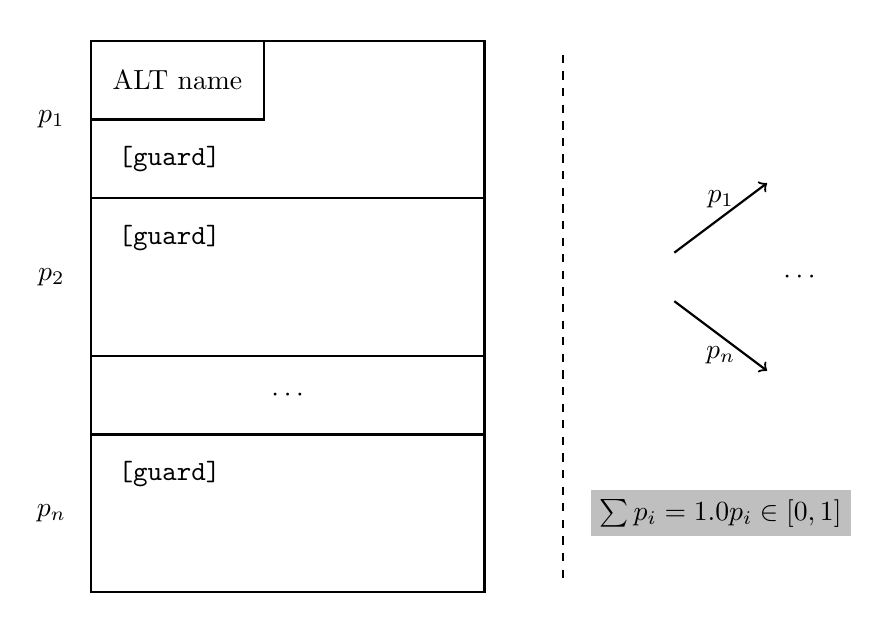
\begin{tikzpicture}[thick]
%%%%%%%%%%%%%%%%%%%%%%%%%%%%%%%%%%%%%%%%%%% HELP LINES
%\draw[help lines] (0,0) grid +(10,10);

%%%%%%%%%%%%%%%%%%%%%%%%%%%%%%%%%%%%%%%%%%% elements
\draw (1,0) rectangle +(5,2);
\node[shape=rectangle, draw=none](p1) at (0.5,6){$p_1$};
\draw (1,2) rectangle +(5,1);
\node[shape=rectangle, draw=none](p2) at (0.5,4){$p_2$};
\draw (1,3) rectangle +(5,2);
\node[shape=rectangle, draw=none](pn) at (0.5,1){$p_n$};
\draw (1,5) rectangle +(5,2);
\node[shape=rectangle, draw=none](ellipsis) at (3.5,2.5){$\cdots$};
\node[circle, draw=none](t1) at (7,7){};
\node[circle, draw=none](t2) at (7,0){};
\node[circle, dashed, minimum size=1cm] (current) at (8,4){};
\node[circle, minimum size=1cm] (a1) at (10,5.5){};
\node[circle, draw=none] (ai) at (10,4){$\cdots$};
\node[circle, minimum size=1cm] (a2) at (10,2.5){};

%%%%% guards and constraints
\node[shape=rectangle, draw=black, minimum height=1cm, minimum width=2.2cm](alt)at(2.1,6.5){ALT name};
\node[shape=rectangle, draw=none](guard1) at (2,5.5) {\texttt{[guard]}};
\node[shape=rectangle, draw=none](guard2) at (2,4.5) {\texttt{[guard]}};
\node[shape=rectangle, draw=none](guard3) at (2,1.5) {\texttt{[guard]}};
\node[shape=rectangle, fill=gray!50, draw=none](constraint) at (9,1) {$\sum p_{i}=1.0$ \\ $p_{i} \in [0,1]$};

%%%%% edges
\draw[dashed] (t1) -- (t2);
\draw[->, thick] (current) -- node[draw=none,above]{$p_1$}(a1);
\draw[->, thick] (current) -- node[draw=none,below]{$p_n$}(a2);
\end{tikzpicture}


}
\end{center}
\caption{Transformation rule for an alternative fragment of an sequence
diagram.}
\label{fig:transAltFrag_SD}
\end{figure}

\paragraph{Alternative fragment \label{par:altFragTransformation}} 
the transformation rule shown by Figure~\ref{fig:transAltFrag_SD} considers the
probabilities assigned by the domain expert to each lane comprising the activity
diagram. The resulting FDTMC is comprised of the current state with as many
newly created outgoing edges and states as the number of lanes. Each edge
assumes its probability value according to its respective lane represented in
the alternative fragment, such that $p_{i} \in [0,1], \sum_{i=1}^{n} p_{i} =
1.0$.

The FDTMC's state-based view represents the moments just before and after the choice of the 
behavioral branch. The current state represents the software's context at
the choice moment while each of its imediately sucessor states represent the
software context just before starting the execution of the behavior of the choosed branch. The edge's probabilities of the FDTMC assume its respective
probabilities given by the domain expert at the alternative fragment. Due the
alternative choice does not involve any interaction between software components
there is no edge from the current to the \texttt{error} state at the FDTMC. 

%%%%%%%%%%%%%%%%%%%%
\begin{figure}[h!]
\begin{center}
%\includegraphics[scale=0.5]{./img/sdTransLoopFrag}
\resizebox{!}{4cm}{
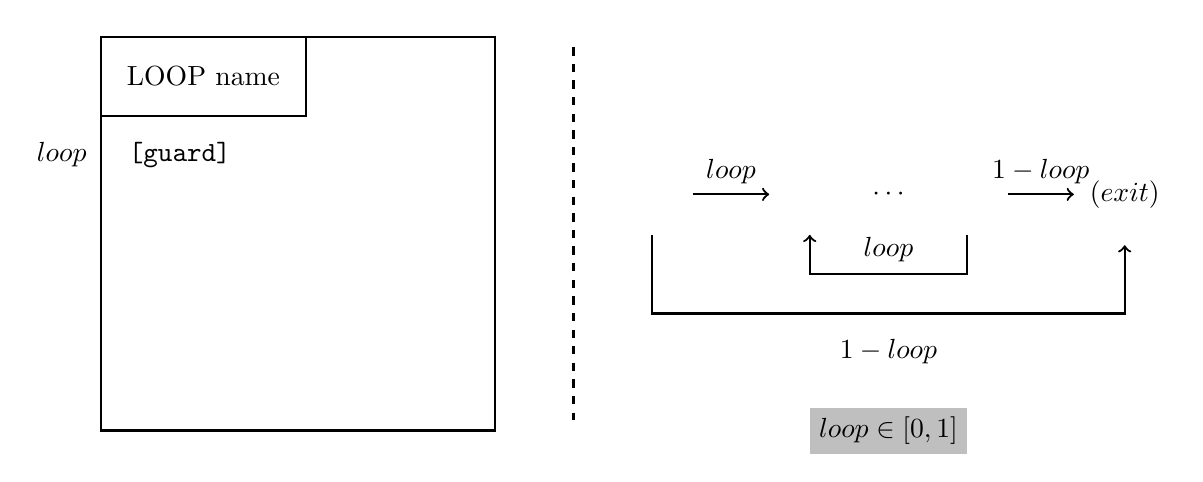
\begin{tikzpicture}[thick]
%%%%%%%%%%%%%%%%%%%%%%%%%%%%%%%%%%%%%%%%%%% HELP LINES
%\draw[help lines] (0,0) grid +(15,10);

%%%%%%%%%%%%%%%%%%%%%%%%%%%%%%%%%%%%%%%%%%% elements
\draw (1,0) rectangle +(5,5);
\node[shape=rectangle, draw=none](p1) at (0.5,3.5){$loop$};
\node[transparent] (t1) at (7,5){};
\node[transparent] (t2) at (7,0){};
\node[circle, dashed, minimum width=1cm] (current) at (8,3){};
\node[circle, minimum width=1cm] (s1) at (10,3){};
\node[circle, draw=none, minimum width=1cm] (s2) at (11,3){$\cdots$};
\node[circle, minimum width=1cm] (s3) at (12,3){};
\node[circle, minimum width=1cm] (s4) at (14,3){($exit$)};
\draw[dashed] (t1) -- (t2);
\draw[->,thick] (current) -- node[draw=none, above]{$loop$}(s1);
\draw[->,thick] (s3) -- node[draw=none, above]{$1-loop$}(s4);
\draw[->,thick] (s3.south) -- +(0,-0.5cm) -| (s1.south);
\node[rectangle, draw=none] at(11,2.3){$loop$};
\draw[->,thick] (current.south) -- +(0,-1cm) -| (s4.south);
\node[rectangle, draw=none] at(11,1){$1-loop$};

%%%%% guards and constraints
\node[shape=rectangle, draw=black, minimum height=1cm, minimum width=2.6cm](alt)at(2.3,4.5){LOOP name};
\node[shape=rectangle, draw=none](guard) at (2,3.5) {\texttt{[guard]}};
\node[shape=rectangle, fill=gray!50, draw=none](constraint) at (11,0) {$loop \in [0,1]$};


\end{tikzpicture}


}
\end{center}
\caption{Transformation rule for a loop fragment of a sequence diagram.}
\label{fig:transLoopFrag_SD}
\end{figure}


\paragraph{Loop fragment:\label{par:loopFragTransformation}}
the FDTMC resulting from the transformation rule shown by
Figure~\ref{fig:transLoopFrag_SD} is comprised of 3 and 4 newly created states and edges
respectively, in addition to the current state. The current state transits to
the second state with the probability given by the parameter \texttt{loop}
defined by the domain expert, or it transits to the \texttt{exit} labeled state
with the complementary probability \texttt{1-loop}.  The analogous reasoning
applies to the third state. The ellipsis between the second and third states
abstracts the resulting FDTMC from the transformation of loop's content. 

%The state-based view for the loop fragment represents the runtime conditions
%the software execution may assume. Albeit the guard-condition is only evaluated
%during the software execution, a domain specialist can define the probability
%of a loop's behavior executes by assigning a value to the \texttt{loop}
%variable.  Once such probability is defined, the first and third FDTMC's states
%turn into choice states as both will enter the loop with the probability given
%by \texttt{loop} or they will leave it with the probability given by
%\texttt{1-loop}.The second and third states represent, respectively, the
%initial state and last state of loop's behavior. Finally, the \texttt{Exit}
%labeled state represents the first reachable state just after the loop
%fragments, i.e., it defines where the software execution continues for the
%first element after the loop fragment.  
The current state represents the software's context whose runtime evaluation
will decide whether the loop fragment will be executed. The first inner state
represents the initial state of the loop's content. The second inner state
indicates the loop's content had executed and another decision about the
iteration must be taken. In case it has to be executed again, the execution
proceeds to the first inner state. Otherwise, it leaves the loop and proceeds to
the first state after the loop content, ie. the \texttt{exit} labeled state.
Such state represents the software is ready to execute the first action just
after the loop fragment.


%%%%%%%%%%%%%%%%%%%%
\begin{figure}[h!]
\begin{center}
%\includegraphics[scale=0.5]{./img/sdTransOptFrag}
\resizebox{!}{4cm}{
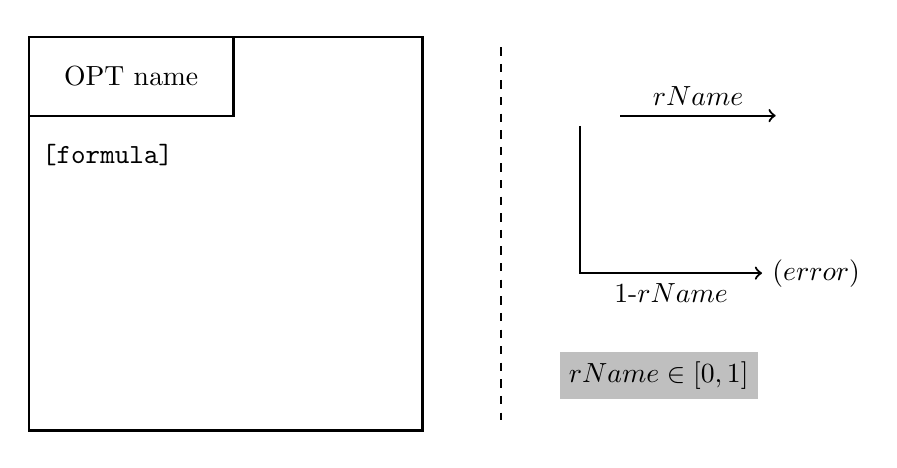
\begin{tikzpicture}[thick]
%%%%%%%%%%%%%%%%%%%%%%%%%%%%%%%%%%%%%%%%%%% HELP LINES
%\draw[help lines] (0,0) grid +(10,10);

%%%%%%%%%%%%%%%%%%%%%%%%%%%%%%%%%%%%%%%%%%% elements
\draw (1,0) rectangle +(5,5);

%%%%% guards and constraints
\node[shape=rectangle, draw=black, minimum height=1cm, minimum width=2.6cm](alt)at(2.3,4.5){OPT name};
\node[shape=rectangle, draw=none](guard) at (2,3.5) {\texttt{[formula]}};

\node[transparent](t1) at (7,5){};
\node[transparent](t2) at (7,0){};
\draw[dashed] (t1) -- (t2);

\node[dashed, minimum width=1cm](current) at (8,4){};
\node[dashed, minimum width=1cm](error) at (11,2){($error$)};
\node[ minimum width=1cm](regular) at (11,4){};
\node[rectangle, draw=none, fill=gray!50](constraint) at (9,0.7){$rName \in [0,1]$};

\draw[->,thick] (current.east) -- node[draw=none, rectangle, above]{$rName$}(regular.west);
\draw[->,thick] (current.south) |- node[draw=none, rectangle, near end, below]{1-$rName$}(error.west);
\end{tikzpicture}

}
\end{center}
\caption{Transformation rule for an optional combined fragment of a sequence
diagram.}
\label{fig:transOptFrag_SD}
\end{figure}

\paragraph{Optional fragment\label{par:optFragTransformation}} 
the transformation rule results into the FDTMC shown by
Figure~\ref{fig:transOptFrag_SD} that is comprised of three states and two
edges, such a state and the edges are newly created by the rule. The current
state transits to the new state with the probability $rName, rName \in [0,1]$
while its complement edge assumes the probability $1-rName$.

The current and the newly created states represent, respectively, the software's
context just before and after the optional fragment execution. Due the resulting
FDTMC represents the optional fragment's reliability, it is agreed the edge's variable
is named as the fragment's name with the `r' prefix standing for reliability.
The \texttt{rName} variable represents the reliability computed for the entire
optional combined fragment in case its behavior is present (ie., for the cases
its guard condition is satisfied). Hence the complement edge represents the
failure probability for executing the optional fragment. In particular, when the
guard condition is not fulfilled by a configuration, the optional fragment's
behavior is not considered part of the product and the \texttt{rName} parameter
assumes the value $1.0$. By assuming such value the complement edge assumes the
probability value $0.0$ that represents there is no failure probability. Indeed,
when the \texttt{rName} assumes the probability value $1.0$ it means there is no
software behavior associated to the edge, thus the optional combined fragment has no effect at the reliability analysis.






%%%%%%%%%%%%%%%%%%%%%%%%%%%%%%%%%%%%%%%%%%%%%%%%%%%%%%%%%%%%%%%%%%%%%%%%%%%%%%%%
%% RELIABILITY EQUIVALENCE OF UML BEHAVIORAL MODELS AND FDTMCs
%%%%%%%%%%%%%%%%%%%%%%%%%%%%%%%%%%%%%%%%%%%%%%%%%%%%%%%%%%%%%%%%%%%%%%%%%%%%%%%%
\section{Reliability Equivalence of UML Behavioral Models and FDTMCs
	\label{sec:reliabilityEquivalenceUMLBehavioralModelsFDTMCs}}


Given a set of UML activity and sequence diagrams representing the  software
product line's behavior, it is possible to compute its reliability by two
distinct manners: a) it can be computed by transforming the UML models into
their respective FDTMCs and then employing state-of-the-art probabilistic model
checkers or b) by applying the reliability functions of each behavioral element
(cf.  Section~\ref{sec:reliabilityUMLBehavioralModels}) in a stepwise fashion
and then traversing the resulting derivation tree solving for a given
configuration.  However, the later evaluation alternative lacks of tools
implementing it whereas, in theory, any parametric and probabilistic model
checker is able to evaluate FDTMCs.  Thus, in order to allow the reuse of existing
and state-of-the-art parametric model checkers, it is necessary to demonstrate
some evidence for the equivalence between reliabilities computed from both UML
and FDTMC models.

\begin{figure}[h!]
\centering
\includegraphics[scale=0.5]{./img/reliabilityEquivalenceIntuition}
\caption{Intuition of the reliability equivalence of UML and FDTMCs models.} 
\label{fig:equivalenceIntuition2}
\end{figure}


Providing a formal proof of the equivalence for reliabilities computed for both
UML and FDTMCs is out of the scope of this work. However some evidences and
arguments presented in the following shows the reliability formulae computed
from both models are equal.  The intuition for such demonstration is depicted
by Figure~3.20.  The elements in boxes represent
behavioral models of a software product line.  Given a UML behavioral model it
is possible to create its respective FDTMC by applying the set of
transformation rules presented at Section~\ref{sec:transformationUMLFDTMC} that
are represented by the leftmost arrow -- the label $T$ represents the set of
transformation rules.  Both dashed arrows leaving the behavioral models
represent a possible reliability evaluation for the software product line.  The
top arrow represents the reliability evaluation of UML behavioral models by the
stepwise application of the reliabilities definitions of
Section~\ref{sec:reliabilityUMLBehavioralModels}. Such evaluation results into
a derivation tree whose terminal nodes denote constants and terms of the
reliability formula such the variables represent the reliabilities of optional
combined fragments.  The bottom edge represents the reliability evaluation of
the FDTMCs resultant from the translation rules applied at the UML behavioral
models.  Such evaluation employs algorithms defined for parametric model
checkers\cite{daws_pmc} resulting into a parametric formula whose parameters
represent the reliabilities values its respective FDTMC may assume.  Thus, to
evidence the equivalence of both reliability evaluations it is necessary
demonstrate the computed reliabilities must be the same when evaluating both
formulae. 


In the next subsections the reliability equivalence of both UML and FDTMCs
models will be demonstrated, using the behavioral models of BSN-SPL represented by the
figures~\ref{fig:bsnControlLoop} and \ref{fig:oxygenationSituation}. 


%%%%%%%%%%%%%%%%%%%%
\subsection{Reliability equivalence for activity diagram
	\label{sec:activityDiagramEquivalence}}

Intuitively, the reliability of a UML behavioral model is given by the
probability of executing all its behavior from the first until the last element
without any error occurrence. According to the
Definition~\ref{eq:behavioralFragmentReliability} it is given by the
accumulated reliability of its first element which, as stated by the
Definition~\ref{eq:accumulatedReliability}, is a recursive function that
considers the accumulated reliability of all elements along the path. Since
each element has its own reliability definition (cf.
Section~\ref{sec:reliabilityOfActivityDiagramModels}), the reliability
computation for a UML activity diagram consists into the stepwise application
of the elements' reliability definitions. Such computation results into a
derivation tree that, when traversed in a pre-order fashion  considering only
terminal nodes and operators, results into its reliability formula. 

Thus, for the case of the activity diagram of the BSN-SPL (represented by
Figure~\ref{fig:bsnControlLoop}), its reliability can be computed by applying
the reliability definitions presented by
Section~\ref{sec:reliabilityOfActivityDiagramModels} until there is no more
node to be expanded by a reliability definition rule, so the
derivation tree is complete. For the sake of space, the stepwise application
rule is not shown, but the whole derivation tree is represented by
Figure~\ref{fig:derivationTreeBSNLoop}. Each derivation step is represented by
an edge linking two nodes containing the reliability definitions for activity
diagram elements with the number of the applied definition rule placed aside.
Finally, the element whose reliability will be computed in the next step (i.e.
the element returned by the \texttt{next} auxiliary function) is shown as a
comment in gray boxes. 

\begin{figure}[htp]
	\centering
	\resizebox{\columnwidth}{!}{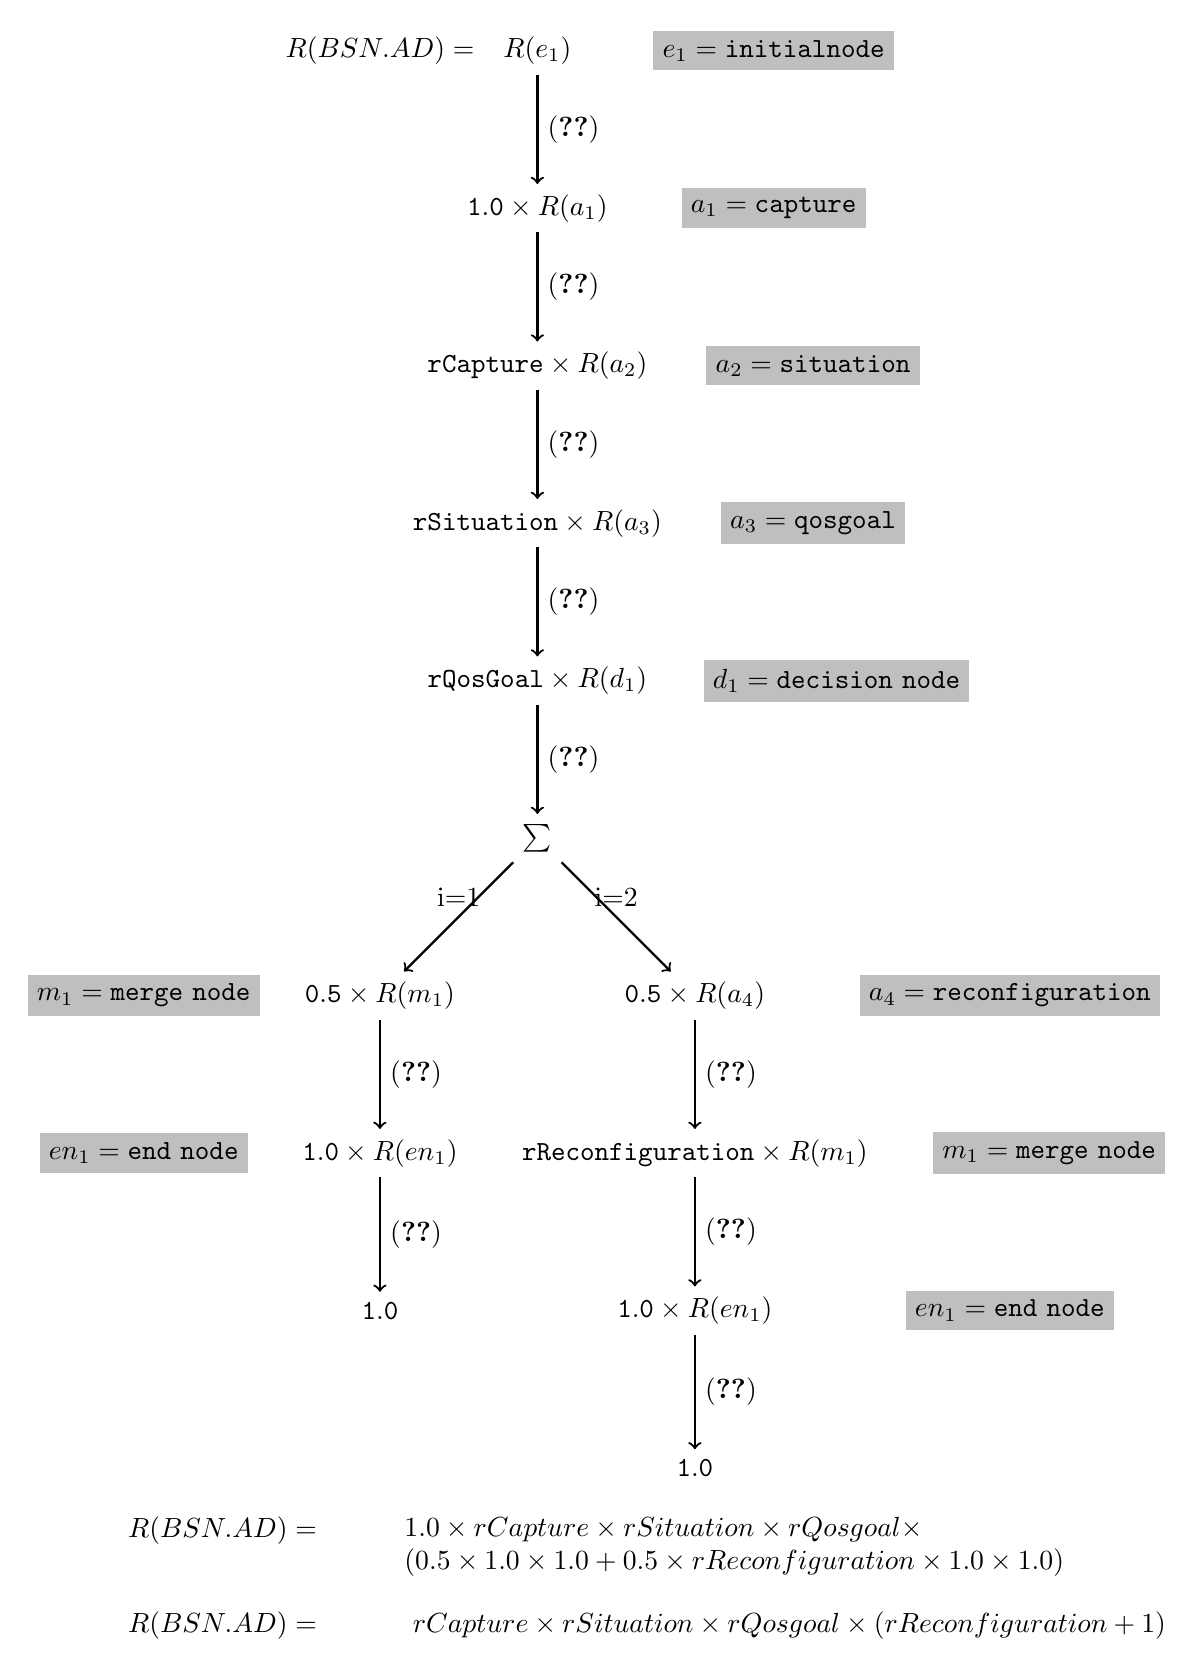
\begin{tikzpicture}[thick]
% \draw[help lines, step=1cm] (0,0) grid +(10,20); 
%%%%%%%%%%%%%%%%%%%%%%%%%%%%%%% Derivation tree for BSN AD
\node[rectangle, draw=none](rBsnAd) at (3.0,20){$R(BSN.AD)=$};
\node[rectangle, draw=none](rinit) at (5,20){$R(e_1)$};
\node[rectangle, draw=none, fill=gray!50](obsBsnAd) at(8,20){$e_1 = \mathtt{initial node}$};
% \draw[->,thick] (rinit) -- node[draw=none,auto]{()}();

\node[rectangle, draw=none](rA1) at (5,18){$\mathtt{1.0} \times R(a_1)$};
\node[rectangle, draw=none, fill=gray!50](obsA1) at(8,18){$a_1 = \mathtt{capture}$};
\draw[->,thick] (rinit) -- node[draw=none,auto]{(\ref{eq:initialNodeReliability})}(rA1);

\node[rectangle, draw=none](rA2) at (5,16){$\mathtt{rCapture} \times R(a_2)$};
\node[rectangle, draw=none, fill=gray!50](obsA2) at(8.5,16){$a_2 = \mathtt{situation}$};
\draw[->,thick] (rA1) -- node[draw=none,auto]{(\ref{eq:activityReliability})}(rA2);

\node[rectangle, draw=none](rA3) at (5,14){$\mathtt{rSituation} \times R(a_3)$};
\node[rectangle, draw=none, fill=gray!50](obsA3) at(8.5,14){$a_3 = \mathtt{qosgoal}$};
\draw[->,thick] (rA2) -- node[draw=none,auto]{(\ref{eq:activityReliability})}(rA3);

\node[rectangle, draw=none](rD1) at (5,12){$\mathtt{rQosGoal} \times R(d_1)$};
\node[rectangle, draw=none, fill=gray!50](obsD1) at(8.8,12){$d_1 = \mathtt{decision\ node}$};
\draw[->,thick] (rA3) -- node[draw=none,auto]{(\ref{eq:activityReliability})}(rD1);

\node[rectangle, draw=none](rSum) at (5,10){$\sum$};
\draw[->,thick] (rD1) -- node[draw=none,auto]{(\ref{eq:decisionNodeReliability})}(rSum);
% \draw[->,thick] () -- node[draw=none,auto]{()}();

\node[rectangle, draw=none](rM1) at (3,8){$\mathtt{0.5} \times R(m_1)$};
\node[rectangle, draw=none, fill=gray!50](obsM1) at(0,8){$m_1 = \mathtt{merge\ node}$};
\draw[->,thick] (rSum) -- node[draw=none,above]{i=1}(rM1);

\node[rectangle, draw=none](rE1) at (3,6){$\mathtt{1.0} \times R(en_1)$};
\node[rectangle, draw=none, fill=gray!50](obsBsnAd) at(0,6){$en_1 = \mathtt{end\ node}$};
\draw[->,thick] (rM1) -- node[draw=none,auto]{(\ref{eq:mergeNodeReliability})}(rE1);

\node[rectangle, draw=none](ren1) at (3,4){$\mathtt{1.0}$};
\draw[->,thick] (rE1) -- node[draw=none,auto]{(\ref{eq:endNodeReliability})}(ren1);

\node[rectangle, draw=none](rA4) at (7,8){$\mathtt{0.5} \times R(a_4)$};
\node[rectangle, draw=none, fill=gray!50](obsA4) at(11,8){$a_4 = \mathtt{reconfiguration}$};
\draw[->,thick] (rSum) -- node[draw=none,above]{i=2}(rA4);

\node[rectangle, draw=none](rM1) at (7,6){$\mathtt{rReconfiguration} \times R(m_1)$};
\node[rectangle, draw=none, fill=gray!50](obsM1) at(11.5,6){$m_1 = \mathtt{merge\ node}$};
\draw[->,thick] (rA4) -- node[draw=none,auto]{(\ref{eq:activityReliability})}(rM1);

\node[rectangle, draw=none](ren1) at (7,4){$\mathtt{1.0} \times R(en_1)$};
\node[rectangle, draw=none, fill=gray!50](obsEn1) at(11,4){$en_1 = \mathtt{end\ node}$};
\draw[->,thick] (rM1) -- node[draw=none,auto]{(\ref{eq:mergeNodeReliability})}(ren1);

\node[rectangle, draw=none](rTerm) at (7,2){$\mathtt{1.0}$};
\draw[->,thick] (ren1) -- node[draw=none,auto]{(\ref{eq:endNodeReliability})}(rTerm);

\node[rectangle, draw=none](rBsnAd) at (1.0,1.2){$R(BSN.AD)= $};
\node[rectangle, draw=none,align=left](rBsnAd) at (7.5,1){$1.0 \times rCapture \times rSituation \times rQosgoal \times $\\$(0.5 \times 1.0 \times 1.0 + 0.5 \times rReconfiguration \times 1.0 \times 1.0) $};
\node[rectangle, draw=none](rBsnAd) at (1.0,0){$R(BSN.AD)= $};
\node[rectangle, draw=none,align=left](rBsnAd) at (8.2,0){$rCapture \times rSituation \times rQosgoal \times ( rReconfiguration + 1) $};

\end{tikzpicture}

}
	\caption{Derivation tree and reliability formula computed for the activity diagram of the BSN-SPL}
	\label{fig:derivationTreeBSNLoop}
\end{figure}

At this point two remarks worth to be addressed regarding the derivation tree
presented by Figure~\ref{fig:derivationTreeBSNLoop}. Initially, it is known the
activity diagram of the BSN-SPL (c.f. Figure~\ref{fig:bsnControlLoop}) has a
common flow of activities until its decision node. Such node splits the
behavior into two execution flows for the cases a reconfiguration is or is not
necessary. Such split is indeed considered in the derivation tree by the
reliability definition~\ref{eq:decisionNodeReliability} for decision nodes,
such from that point the derivation tree also splits in two branches. The
second remark regards to the formula resulting from the tree traversal in a
pre-order fashion. By considering the terms and operators of each node the
reliability for such activity diagram is given by the formula $R(BSN.AD)= 1.0
\times rCapture \times rSituation \times rQosgoal \times $\\$(0.5 \times 1.0
\times 1.0 + 0.5 \times rReconfiguration \times 1.0 \times 1.0) $ that, in its
simplified form, is equals to $R(BSN.AD)= 0.5\times  rCapture \times rSituation \times
rQosgoal \times ( rReconfiguration + 1)$. In such formula, the common flow of
activities reflects into the multiplication of the four initial terms,
meanwhile the decision node is the responsible for generating the sum of
$(rReconfiguration + 1)$. As the decision node is part of the execution flow,
its sum is multiplied by the multiplication related to the common flow (i.e.
the three initial activities and the decision's node probability). 

\begin{figure}[htp]
	\centering
	\resizebox{\columnwidth}{!}{\begin{tikzpicture}[x=1.5cm]
\centering
%%%%%%%%%%%%%%%%%%%%%%%% help lines
%\draw[help lines] (0,0) grid +(6,2);

%%%%%%%%%%%%%%%%%%%%%%%% nodes
\node[initial](initial) at (-1,1) {(\textit{init})};
\node[](firs) at (0,1){};
\node[](capt) at (1,1){};
\node[](situ) at (2,1){};
\node[](qosg) at (3,1){};
\node[](deci) at (4,1){};
\node[](reco) at (5,1){};
\node[](merg) at (6,1){};
\node[](success) at (7.5,1){(\textit{success})};
\node[](error) at (7.5,-1){(\textit{error})};

%%%%%%%%%%%%%%%%%%%%%%%% edges
\draw[thick, -{latex[width=3mm]}] (initial) to node[draw=none, rotate=45, yshift=0.6cm, xshift=0.8cm]{\scriptsize $1.0$} (firs);
\draw[thick, -{latex[width=3mm]}] (firs) to node[draw=none, rotate=45, yshift=0.6cm, xshift=0.8cm]{\scriptsize $rCapture$}  (capt);
\draw[thick, -{latex[width=3mm]}] (capt) -- node[draw=none, rotate=45, yshift=0.6cm, xshift=0.8cm]{\scriptsize $rSituation$} (situ);
\draw[thick, -{latex[width=3mm]}] (situ) --  node[draw=none, rotate=45, yshift=0.6cm, xshift=0.8cm]{\scriptsize $rQosGoal$}(qosg);
\draw[thick, -{latex[width=3mm]}] (qosg) --  node[draw=none, rotate=45, above, xshift=0.3cm]{\scriptsize $0.5$}(deci);
\draw[thick, -{latex[width=3mm]}] (deci) --  node[draw=none, rotate=45, yshift=0.4cm, xshift=1.2cm]{\scriptsize $rReconfiguration$}(reco);
\draw[thick, -{latex[width=3mm]}] (reco) --  node[draw=none, rotate=45, yshift=0.4cm, xshift=0.2cm]{\scriptsize $1.0$}(merg);
\draw[thick, -{latex[width=3mm]}] (merg) --  node[draw=none, rotate=45, yshift=0.4cm, xshift=0.2cm]{\scriptsize $1.0$}(success);
\draw[thick, -{latex[width=3mm]}] (qosg) -- +(0,2cm) -|  node[draw=none, rotate=45, above, near start]{\scriptsize $0.5$} (merg);
\path[-{latex[width=3mm]}] (success) edge [loop right] node [draw=none]{$1.0$}();

\draw[thin, ->](initial) |- node[draw=none, rotate=45]{$0.0$}(error);
\draw[thin, ->](firs) |- node[draw=none, rotate=45]{$1-rCapture$}(error);
\draw[thin, ->](capt) |- node[draw=none, rotate=45]{$1-rCapture$}(error);
\draw[thin, ->](situ) |- node[draw=none, rotate=45]{$1-rSituation$}(error);
\draw[thin, ->](qosg) |- node[draw=none, rotate=45]{$1-rQosGoal$}(error);
\draw[thin, ->](deci) |- node[draw=none, rotate=45]{$1-rReconfiguration$}(error);
\draw[thin, ->](reco) |- node[draw=none, rotate=45]{$0.0$}(error);
\draw[thin, ->](merg) |- node[draw=none, rotate=45]{$0.0$}(error);
\end{tikzpicture}

}
	\caption{FDTMC the activity diagram of the BSN-SPL}
	\label{fig:fdtmcBSNLoop}
\end{figure}

The other manner to compute the reliability of the activity diagram is to apply
the transformations from UML to FDTMC substructures defined for activity
diagram elements in Section~\ref{subsec:transfomrationRulesActivityDiagramElements} in
stepwise fashion and then evaluate the resulting FDTMC by means of a parametric
model checker. Since the reliability is the property of interest, it can
defined as the probability of reaching the FDTMC's final state labeled as
``success''by the PCTL statement $P_{=?}(\Diamond ''success'')$. Again, for the
sake of space the stepwise construction of the FDTMC is not shown, but the
resulting FDTMC is shown by Figure~\ref{fig:fdtmcBSNLoop}. In such FDTMC, it is
possible to infer that only two possible paths lead to the success state. Both
paths have the initial four transitions and, from the fifth state, the
execution splits into two possible paths. Such splitting stems from the
transformation rule~\ref{fig:transDecis_AD} defined for decision nodes of
activity diagrams. Later, such paths merges into a common flow at the $8^{th}$
state, as defined by the transformation rule~\ref{fig:transMerge_AD}. According
to the reliability definition provided by \citet{grunske_specification_2008},
the reliability can be computed by a rechability measure in a probabilistic
model that, intuitively, is defined as the sum of probabilities computed for
each possible execution path of a probabilistic
model\cite{baier_principles_2008}. When a parametric model checker's
algorithm\cite{daws_pmc} is employed to verify the aforementioned PCTL
statement at the FDTMC shown by Figure~\ref{fig:fdtmcBSNLoop} the resulting
formula for its reliability is equal to $1.0 \times rCapture \times
rSituation \times rQosgoal \times 0.5 \times 1.0 + 1.0 \times rCapture
\times rSituation \times rQosgoal \times 0.5 \times rReconfiguration \times
1.0 \times 1.0 $, where the variables starting with 'r' denotes the reliability
of its related activity. Such formula, in its simplified form, is equals to
$0.5 \times rCapture \times rSituation \times rQosgoal \times (rReconfiguration
+ 1)$.

Albeit the UML activity diagram and its related FDTMC describes different
characteristics of the BSN-SPL (the activity diagram provides the action-based
view meanwhile the FDTMC the state-based view), the reliability formulae
computed from both models are equals. Despite it is not a formal demonstration
of reliability equivalence between such models, the equality of such formulae
provides evidences that the reliability of a UML behavioral model can be
computed by employing algorithms of parametric model checkers into its related
FDTMC. In addition, such demonstration also provides evidences that the
transformation rules for activity diagram elements (cf.
Section~\ref{subsec:transfomrationRulesActivityDiagramElements} are correct in
the sense they preserve the reliability notion of the considered elements.



%%%%%%%%%%%%%%%%%%%%
\subsection{Reliability equivalence for sequence diagram
	\label{sec:sequenceDiagramEquivalence}}
%
To present evidences that a UML Sequence Diagram and its respective FDTMC have
reliability equivalence, the demonstration's intuition represented by
Figure~\ref{fig:reliabilityEquivalenceIntuition} is still valid. Its rationale
is to show that both models, when analyzed with their suitable evaluation
method, will converge to a common reliability formula. The implications of
such formulae convergence are threefold. Initially, it implies the reliability
of a software represented by a UML Sequence Diagram can be evaluated by its
respective FDTMC so taking advantages of the state-of-the art model checkers.
In addition, it evidences the semantics of software reliability is preserved by
an \emph{activity-based} and its respective \emph{state-based} models. Finally,
it indicates the transformation rule's correctness since the FDTMC build by the
stepwise application of transformation rules preserves the semantics of its
original UML Sequence Diagram.

To demonstrate the reliability equivalence the sequence diagram ``System
identifies \underline{situation}'' shown by
Figure~\ref{fig:oxygenationSituation} will be used as a running example. Such
diagram is chosen due it is representativeness given the range of elements
comprising its behavior.


%%%%%%%%%%
%\paragraph{System identifies situation}
%
%The activity ``\textit{System identifies situation}'' is responsible to compute
%the individual's health situation based on the information gathered from the
%sensors. The individual's health situation is computed based on five vital
%signals namely oxygenation, temperature, pulse rate, positioning and if the
%individual falled. Each signal processing is represented by its own sequence
%diagram such there are 5 sequence diagrams sequentially associated to the
%activity ``\textit{System identifies situation}''.  Oxygenation is the first
%vital signal to be processed and its behavior is represented by Figure
%\ref{fig:oxySD}. 
%
%\begin{figure}[h!]
%	\textit{\textbf{Place oxygenation's sequence diagram.}}
%	\caption{Sequence diagram for processing the oxygenation information.}
%	\label{fig:oxySD}
%\end{figure}
%
%Briefly, the behavior for processing the oxygenation information consists of
%interactions between the software component \texttt{Oxygenation}, the
%persistence components \texttt{Persistence}, \texttt{SQlite} and
%\texttt{Memory}, and the \texttt{Bus} that is responsible by addressing the
%inter-components communications. The oxygenation's behavior has two variability
%points that allow persist its data in an SQlite database or in memory. 

The first element to transform is the synchronous message \texttt{register}
whose $0.999$ associated value denotes the communication channel's reliability.
As the sequence diagram's reliability is the cummulated reliability of its first
element, Definition \ref{eq:syncMessageReliability} is applied such: 

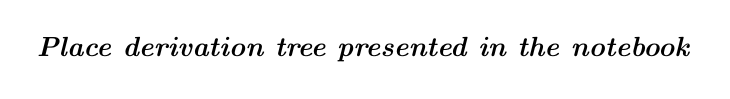
\begin{tikzpicture}[
		    every node/.style={draw=none},
	]
	\node{\textit{\textbf{Place derivation tree presented in the notebook}}};	
\label{dt:register}
\end{tikzpicture}

where $SD$ is the sequence diagram, $e_1$ is the \texttt{register} message and
$E_1 = [E \backslash e_1]$ is the elements list resulting from removing $e_1$
from the list $E$ containing all elements.

Once the \texttt{register} message is addressed and removed from the elements
list $E$, the reliability analysis proceed with the remaining elements, as $E_1$
in the derivation tree above represents the resulting list. In the next step,
the list's first element is the \texttt{reply} message associated to
\texttt{register}.  When definition \ref{eq:replyMessageReliability} is applied
results into the derivation tree

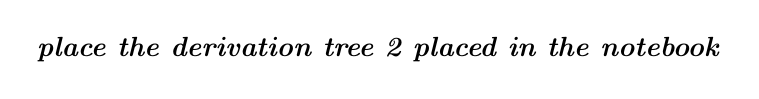
\begin{tikzpicture}[
	every node/.style={draw=none}]
\node{\textit{\textbf{place the derivation tree 2 placed in the notebook}}};
\label{dt:registerReply}
\end{tikzpicture}

where $e_2$ is the reply message and $E_3=[E_2 \backslash e_2]$.

From the derivation tree above, the remaining list $E_2$ starts with the
assynchronous message \texttt{sendSituation(spo2Situation)}. Thus, when the
reliability definition \ref{eq:assyncMessageReliability} is applied over $E_2$,
it results into the following derivation tree

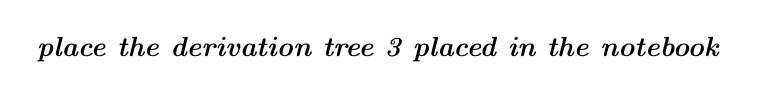
\begin{tikzpicture}
	[
		every node/.style={draw=none}
	]
\node{\textbf{\textit{place the derivation tree 3 placed in the notebook}}};
\label{dt:sndSituationAssync}
\end{tikzpicture}
where $e_2$ is the assynchronous message \texttt{sendSituation} and $E_3 =
[E_2 \backslash e_2]$ is the remaining list. 

The first element of the list $E_3$ is the synchronous message \texttt{persist}
directed to the software component responsible to persist data in different
manners. Thus, when the reliability definition~\ref{eq:syncMessageReliability}
is applied at $E_3$ it results into the following derivation tree

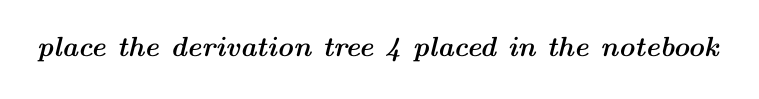
\begin{tikzpicture}
	[
		every node/.style={draw=none}
	]
\node{\textbf{\textit{place the derivation tree 4 placed in the notebook}}};
\label{dt:persistAssync}
\end{tikzpicture}

where $e_3$ is the assynchronous message and $E_4 = [E_3 \backslash e_3]$ is the list
containing the remaining elements after removing $e_3$ from $E_3$. 

The resulting list $E_4$ has as its first element the optional combined fragment
representing the behavior associated to the SQLite feature. According to the
reliability definition~\ref{eq:optionalFragmentReliability}, the reliability of the
optional fragment is represented by a single parameter, whose value will be
computed later. Since the element after the fragment representing the SQLite's
behavior is another combined fragment, for the sake of space, the derivation
tree shown below results from the twice application of
Definition~\ref{eq:optionalFragmentReliability} 

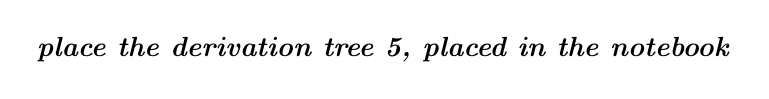
\begin{tikzpicture}
	[
		every node/.style={draw=none}
	]
\node{\textbf{\textit{place the derivation tree 5, placed in the notebook}}};
\label{dt:optSqliteMemory}
\end{tikzpicture}

where $e_6$ is the optional fragment associated to \texttt{SQLite} feature,
$E_6=[E_5 \backslash e_6 ]$, $e_7$ is the optional fragment associated to
\texttt{Memory} feature and $E_7 = [E_6 \backslash e_6]$ is the list containing
the remaining elements. 

At this point the $E_7$ list has the \texttt{reply} message (associated to
\texttt{persist} synchronous message) as its first element. Since the
reliability definition of a reply message is given by
\ref{eq:replyMessageReliability}, when it is applied it results into the
derivation tree

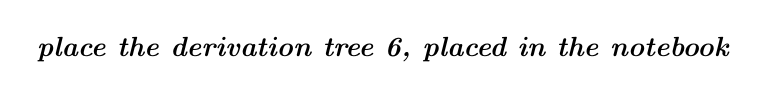
\begin{tikzpicture}
	[
		every node/.style={draw=none}
	]
\node{\textit{\textbf{place the derivation tree 6, placed in the notebook}}};
\label{dt:replyPersist}
\end{tikzpicture}

where $e_8$ is the reply message associated to the persist message and $E_8 =
[E_7 \backslash e_8]$ is the list of the remaining elements. 

At this point the $E_8$ contains the \texttt{sendSituation()} assynchronous
message as its first element, whose reliability definition is given by
\ref{eq:assyncMessageReliability}. Its application over the sequence diagram
results 

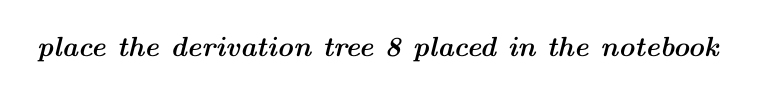
\begin{tikzpicture}
	[
		every node/.style={draw=none}
	]
\node{\textit{\textbf{place the derivation tree 8 placed in the notebook}}};
\label{dt:sndSituationAssync2}
\end{tikzpicture}

where $e_{10}$ is the reply message and $E_{10} = [E_9 \backslash e_{10}]$ is
the set of remaining elements after removing $e_{10}$ from $E_9$. 

Finally, the last iteration of the reliability function $R$ is over $E_{10}$
which is an empty list since all elements were already addressed. As the empty
list has no associated behavior, its reliability is $1.0$ by definition. Thus,
the derivation tree for $E_{10}$ is

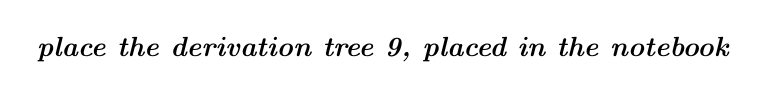
\begin{tikzpicture}
	[
		every node/.style={draw=none}
	]
\node{\textbf{\textit{place the derivation tree 9, placed in the notebook}}};
\label{dt:emptyList}
\end{tikzpicture}

Since there is no more element in the remaining elements list that represents
the sequence diagram, the resultant derivation tree is complete and it is shown
below.

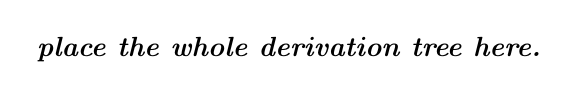
\begin{tikzpicture}
	[
		every node/.style={draw=none}
	]
\node{\textbf{\textit{place the whole derivation tree here.}}};
\label{dt:wholeDT}
\end{tikzpicture}

Since the sequence diagram's reliability is given by the cummulated reliability
of its first element, as stated by Definition~\ref{}, it can be computed by
traversing the derivation tree~\ref{dt:wholeDT} in a pre-order fashion. Thus,
the result for such traversal is 
\begin{align}
R(Oxygenation) = &0.999 \times 0.999 \times 0.999 \times 0.999 \times rSqlite
\times \nonumber \\ &rMem \times 0.999 \times 0.999 \times 0.999 \nonumber \\
               = &0.999^7 \times rSqlite \times rMem
\label{eq:situationActivityDiagramReliability}
\end{align}

where the $rSqlite$ and $rMem$ are the variables that represent the
reliabilities of the optional fragments representing the behavior of SQLite and
Memory features, respectively.

Once \ref{eq:situationActivityDiagramReliability} is computed from the
reliability function $R$ applied at the activity diagram, it is necessary to
create its respective FDTMC by applying the transformation rules for sequence
diagram elements defined at
Section~\ref{sec:sequenceDiagramTransformationRules}. When the FDTMC building
is finished, its reliability can be computed by using the well-known reliability
definition provided by \cite{grunske_specification_2008} and the reachability
measure definition provided by \cite{baier_principles_2008}. 

The FDTMC building is accomplished in a stepwise fashion and follows the
partial-ordering of the set of sequence diagram elements. When an element is
transformed by its corresponding rule, its resulting FDTMC substructure is added
to the FDTMC created by previous transformation rules from the \textit{current state}. In the case of the "System
identifies \underline{situation}" sequence
diagram, the first element to be transformed is the \texttt{register}
synchronous message. When its transformation rule is applied (cf.
Figure~\ref{fig:transSync_SD}), the resulting FDTMC comprises the initial, error
and a new state besides two transitions, as shown by Figure \ref{xxx}.

\begin{figure}
\textbf{\textit{Place the FDTMC 1, depicted in the notebook.}}
\caption{FDTMC resulting from the transformation of \texttt{register} message.}
\label{fig:fdtmcRegister}
\end{figure}

The next element to be transformed, according to the sequence diagram's
partial-ordering is the \texttt{reply} message associated to the
\texttt{register} message. The transformation rules represented at
Figure~\ref{fig:trasReply_SD} builds a state and two edges newly created from
the current state, so results into the FDTMC shown by
Figure~\ref{fig:fdtmcRegisterReply}.

\begin{figure}
\textbf{\textit{Place the FDTMC 2, depicted in the notebook.}}
\caption{FDTMC resulting from the transformation of \texttt{reply} message.}
\label{fig:fdtmcRegisterReply}
\end{figure}

In the sequence, the \texttt{sendSituation} assynchronous message is transformed
into an FDTMC from the current state by the transformation rule represented at
Figure~\ref{fig:transAssync_SD}. The transformation adds a state and two states
newly created, as shown by Figure~\ref{fig:fdtmcSendSituation}.

\begin{figure} 
	\textbf{\textit{Place the FDTMC 3, depicted in the notebook.}}
	\caption{FDTMC resulting from the transformation of
	\texttt{sendSituation} message.} 
	\label{fig:fdtmcSendSituation}
\end{figure}

The next element to transform is the synchronous message \texttt{persist}. So
when its transformation is applied a state and two new edges are added from the
current state, that results the FDTMC shown by Figure~\ref{fig:fdtmcPersistSync}.

\begin{figure} 
	\textbf{\textit{Place the FDTMC 4, depicted in the notebook.}}
	\caption{FDTMC resulting from the transformation of \texttt{persist}
	message.} 
	\label{fig:fdtmcPersistSync}
\end{figure}

The next element to be transformed is the optional combined fragment
representing the behavior of SQLite feature. According to
Figure~\ref{fig:transOptFrag_SD} the transformation adds a state and two edges
newly created. The reliability of the fragment's internal sequence diagram is
represented on both created edges by the \texttt{rSqlite} variable, whose value
will be evaluated later. Since the next element is another optional combined
fragment that represents the memory feature's behavior, the analogous rationale
is valid such the transformation represented by Figure~\ref{fig:transOptFrag_SD}
is applied again. The result of such transformations is represented by
Figure~\ref{fig:fdtmcSqliteMemory}, where the elements added by both
transformations are distinguished from the existing elements for being
represented in solid lines.

\begin{figure} 
	\textbf{\textit{Place the FDTMC 5, depicted in the notebook.}}
	\caption{FDTMC resulting from the transformation of \texttt{SQLite} and
	\texttt{Memory} optional combined fragments.}
	\label{fig:fdtmcPersistSync}
\end{figure}

The next element to transform is the reply message associated to the
\texttt{persist}
synchronous message. When the transformation represented at
Figure~\ref{fig:transReply_SD} is applied it results into the FDTMC represented
by the Figure~\ref{fig:fdtmcReplyPersist}.

\begin{figure} 
	\textbf{\textit{Place the FDTMC 6, depicted in the notebook.}}
	\caption{FDTMC resulting from the transformation of \texttt{reply}
	message associated to the \texttt{persist} message.}
	\label{fig:fdtmcReplyPersist}.
\end{figure}

In the following the interaction between the \texttt{Oxygenation} and
\texttt{Bus} software components, comprised of the \texttt{sendSituation} and its return,
is transformed into a FDTMC substructure by applying the transformations for
\texttt{assynchronous} and \texttt{reply} message, in this sequence. The
resulting FDTMC is build by first adding a state and two edges newly created
from the current state, as defined by transformation of assynchronous rule
represented by Figure~\ref{fig:transAssync_SD}. From the new current state, the
FDTMC substructure corresponding to the reply message is build, by adding a
state and two newly created edges. As there is no other element to be
transformed, the current state is considered the FDTMC's last state to be reach
in case no error occur during the execution. Thus, it is labeled as ``success''
and transformed into an absorbing state by the auto-edge with $1.0$ as the
probability value. The Figure~\ref{fig:fdtmcSndSituationReply} is the final
FDTMC for the ``System identifies situation'' sequence diagram. 

\begin{figure} 
	\textbf{\textit{Place the FDTMC 7, depicted in the notebook.}}
	\caption{FDTMC resulting from the transformation of
		\texttt{sendSituation} and its corresponding \texttt{reply}
		message.}
	\label{fig:fdtmcReplyPersist}.
\end{figure}









For such FDTMC it is possible to apply the reachability measure
algorithm\cite{baier_principles_2008} in order to compute its
reliability\cite{grunske_specification_2008}. As
the FDTMC is comprised of a unique path from the \texttt{initial} to the
\texttt{sucess} state, the evaluation of the reliability property
$P=\Diamond(``sucess'')$ of the whole sequence diagram is equal to the
product of all probabilities along the path, including the parameters that
represent the reliabilities of the optional combined fragments.
Thus, such evaluation results into the following formula.

\scriptsize
\begin{align}
rOxygenation =&0.999 \times 0.999 \times 0.999 \times 0.999 \times rSqlite \times
rMemory \times 0.999 \times 0.999 \times 0.999 \times 0.999 \nonumber \\
rOxygenation =&0.999^7 \times rSQLite \times rMemory
\label{eq:oxygenationFDTMCReliability}
\end{align}
\normalsize

Given that \ref{eq:captureFDTMCReliability} denotes the reliability computed
from the FDTMC built from the transformation of the sequence diagram associated
to the ``System identifies situation'' activity, it is possible to analyse the
equivalence intuition depicted by
Figure~\ref{fig:reliabilityEquivalenceIntuition} in order to gather some
evidence concerning the reliabilities equivalence. In a brief, the sequence
diagram's reliability was computed by applying the reliability definitions for
each element in a stepwise fashion, which results into the reliability
formula~\ref{eq:situtationActivityDiagramReliability}. By the other side, the
sequence diagram was transformed into a FDTMC by applying the transformation
rules shown at Section~\ref{sec:sequenceDiagramTransformationRules}. The FDTMC
was evaluated by a well-known reachability algorithm which resulted the
formula~\ref{eq:oxygenationFDTMCReliability}. Both reliability formulae are
equals albeit they were computed using different methods, which provides the
evidence that the reliability of a sequence diagram and its FDTMC are
equivalent. In addition, as the FDTMC is build based on the transformation rules
and the FDTMC's reliability is equivalent to the sequence diagram's reliability,
it also provides the confidence that the transformation rules employed are also
correct.

Finally, it is important mention the behavioral variability of the ``System
identifies situation'' and its impact over its reliability. The behavior of
such sequence diagram is variable according to the optional combined fragments
which it comprises. By your turn, each combined fragment will only be executed
for the configurations which satisfy its guard condition. Thus, every time one
of its optional combined fragment is executed, its respective variable in the
formula~\ref{eq:oxygenationFDTMCReliability} assumes its reliability value. In
case its guard condition is not satisfied, its impact over the reliability of
the whole sequence diagram is null and, as the reliability given by
\ref{eq:captureFDTMCReliability} is a formula whose terms are products of of
reliabilities, its respective variable assumes $1.0$ as reliability value so it
does not affect the reliability computation. 



Once the demonstration presented in
Section~\ref{sec:activityDiagramEquivalence} provides evidences there is
equivalence of reliabilities computed from UML activity diagram and its related
FDTMC, it is necessary obtain similar evidences for UML sequence diagram and
its FDTMC. Thus, the demonstration's intuition represented in
Figure~3.20 still holds  and the notation used to
represent the derivation tree will also be used for the reliability definitions
of sequence diagrams. 

\begin{figure}[htp]
	\centering
	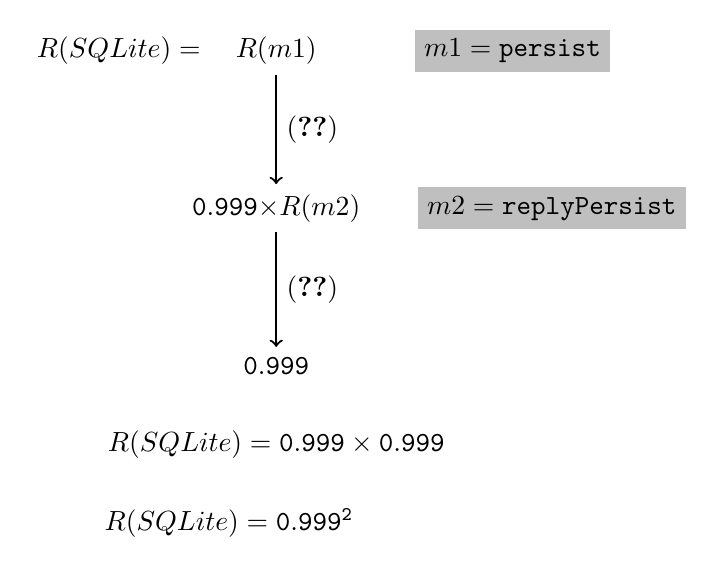
\begin{tikzpicture}[thick]
%\draw[help lines, step=1cm] (0,0) grid +(10,15);
%%%%%%%%%%%%%%%%%%%%%%%%%%%%%%% Derivation tree for SQLite
\node[rectangle, draw=none](rSqlite) at (0,15){$R(SQLite)=$};
\node[rectangle, draw=none](rM1) at (2,15){$R(m1)$};
\node[rectangle, draw=none, fill=gray!50](obsM1) at(5,15){$m1 = \mathtt{persist}$};
\node[rectangle, draw=none](rM2) at(2,13){$\mathtt{0.999 \times} R(m2)$};
\node[rectangle, draw=none, fill=gray!50](obsM1) at(5.5,13){$m2 = \mathtt{replyPersist}$};
\draw[->, thick] (rM1) -- node[draw=none, auto]{(\ref{eq:syncMessageReliability})}(rM2);
\node[rectangle, draw=none](rTerm) at(2,11){$\mathtt{0.999}$};
\draw[->, thick] (rM2) -- node[draw=none, auto]{(\ref{eq:syncMessageReliability})}(rTerm);
\node[rectangle, draw=none](rSqlite) at (2,10){$R(SQLite)= \mathtt{0.999 \times 0.999}$};
\node[rectangle, draw=none](rSqlite) at (1.4,9){$R(SQLite)= \mathtt{0.999^2}$};
\end{tikzpicture}

	\caption{Derivation tree of reliability definitions for the \emph{Sqlite} feature}
	\label{fig:derivationTreeSqliteMemory}
\end{figure}

Figure~\ref{fig:derivationTreeSqliteMemory} presents the derivation tree of the
fragment \texttt{rSqlite} presented in the
Figure~\ref{fig:oxygenationSituation}. Since the behavior of such fragment is
represented by its inner sequence diagram and such diagram does not have any
variability point, the demonstration related in the following also holds for all
sequence diagrams that does not have variability points. Such fragment
comprises a synchronous and its reply message for the data persistence. Thus,
the reliability definition~\ref{eq:syncMessageReliability} is applied twice
resulting into the derivation tree
(Figure~\ref{fig:derivationTreeSqliteMemory}. Since the sequence diagram does
not have variability points its resulting reliability formula is given in terms
of constants. Thus, the reliability computed for such fragment is $R(SQLite) =
0.999^2$.

\begin{figure}[htp]
	\centering
	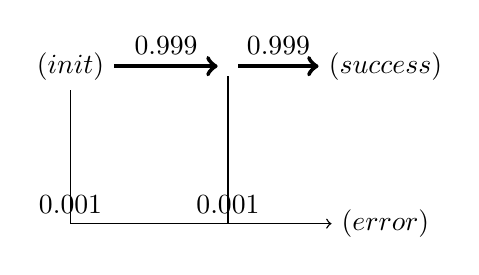
\begin{tikzpicture}[thick]
%\draw[help lines, step=1cm] (0,0) grid +(10,15);
%%%%%%%%%%%%%%%%%%%%%%%%%%%%%%% FDTMC for SQLite
\node(init) at (0,7){$(init)$};
\node(s1) at (2,7){};
\node(success) at (4,7){$(success)$};
\node(error) at (4,5){$(error)$};
\draw[->, ultra thick] (init) -- node[draw=none, above]{0.999}(s1);
\draw[->, ultra thick] (s1) -- node[draw=none, above]{0.999}(success);
\draw[->,auto, thin] (init) |- node[draw=none, above]{0.001}(error);
\draw[->,auto, thin] (s1) |- node[draw=none, above]{0.001}(error);
\end{tikzpicture}

	\caption{FDTMC of the \emph{Sqlite} feature}
	\label{fig:fdtmcEquivalenceSqliteMemory}
\end{figure}

In the case of the reliability analysis by means of a model checker,
the FDTMC for the fragment is build by applying the transformation
rule~\ref{fig:transSync_SD} twice, then resulting the structure shown by
Figure~\ref{fig:fdtmcEquivalenceSqliteMemory}. When the property
$P_{?=}(\Diamond ''success'')$is evaluated by a parametric model checker, its
resulting formula is $0.999 \times 0.999$, thus equals to the reliability
formula computed from its respective sequence diagram. 


\begin{figure}[htp]
	\centering
	\resizebox{\columnwidth}{!}{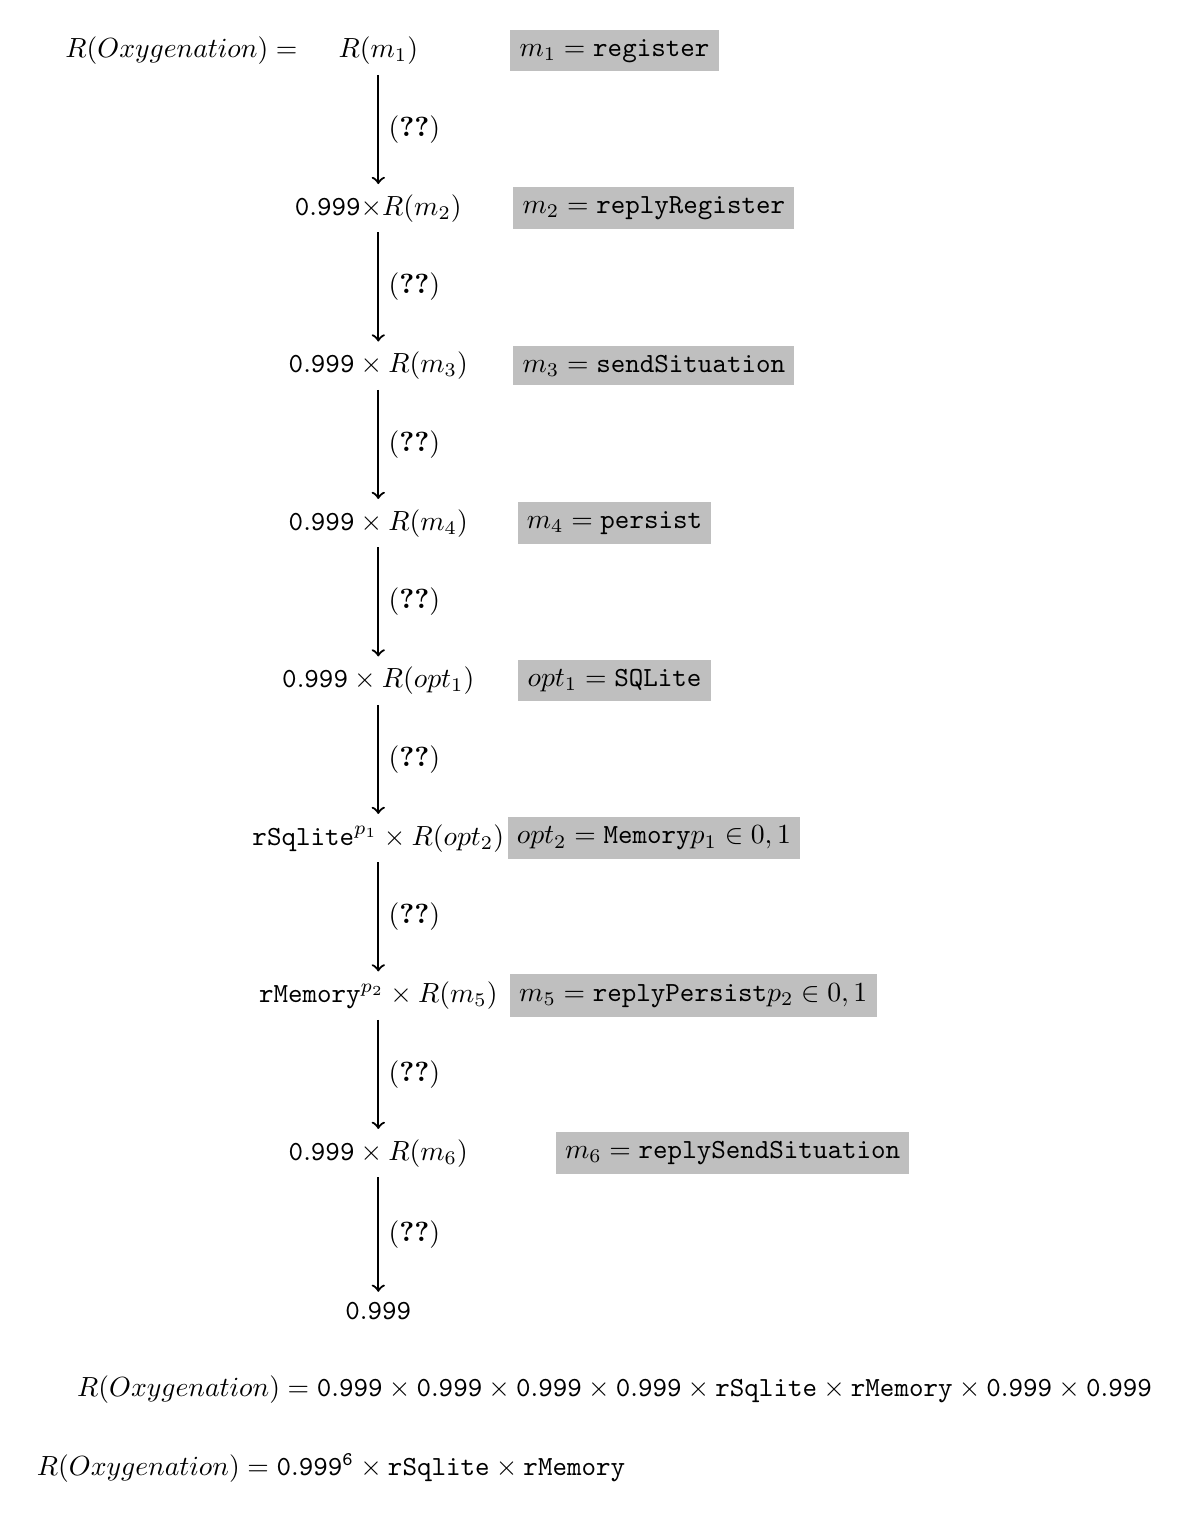
\begin{tikzpicture}[thick]
%\draw[help lines, step=1cm] (0,0) grid +(10,15);
%%%%%%%%%%%%%%%%%%%%%%%%%%%%%%% Derivation tree for SQLite
\node[rectangle, draw=none](rOxygenation) at (-0.5,15){$R(Oxygenation)=$};
\node[rectangle, draw=none](rM1) at (2,15){$R(m_1)$};
\node[rectangle, draw=none, fill=gray!50](obsM1) at(5,15){$m_1 = \mathtt{register}$};
\node[rectangle, draw=none](rM2) at(2,13){$\mathtt{0.999 \times} R(m_2)$};
\node[rectangle, draw=none, fill=gray!50](obsM1) at(5.5,13){$m_2 = \mathtt{replyRegister}$};
\draw[->, thick] (rM1) -- node[draw=none, auto]{(\ref{eq:syncMessageReliability})}(rM2);
\node[rectangle, draw=none](rM3) at(2,11){$\mathtt{0.999} \times R(m_3)$};
\node[rectangle, draw=none, fill=gray!50](obsM1) at(5.5,11){$m_3 = \mathtt{sendSituation}$};
\draw[->, thick] (rM2) -- node[draw=none, auto]{(\ref{eq:syncMessageReliability})}(rM3);

\node[rectangle, draw=none](rM4) at(2,9){$\mathtt{0.999} \times R(m_4)$};
\node[rectangle, draw=none, fill=gray!50](obsM4) at(5,9){$m_4 = \mathtt{persist}$};
\draw[->, thick] (rM3) -- node[draw=none, auto]{(\ref{eq:syncMessageReliability})}(rM4);
\node[rectangle, draw=none](rOpt1) at(2,7){$\mathtt{0.999} \times R(opt_1)$};
\node[rectangle, draw=none, fill=gray!50](obsOpt1) at(5,7){$opt_1 = \mathtt{SQLite}$};
\draw[->, thick] (rM4) -- node[draw=none, auto]{(\ref{eq:syncMessageReliability})}(rOpt1);
\node[rectangle, draw=none](rOpt2) at(2,5){$\mathtt{rSqlite}^{p_1} \times R(opt_2)$};
\node[rectangle, draw=none, fill=gray!50](obsOpt2) at(5.5,5){$opt_2 = \mathtt{Memory}$\\$p_1 \in {0,1}$};
\draw[->, thick] (rOpt1) -- node[draw=none, auto]{(\ref{eq:optionalFragmentReliability})}(rOpt2);
\node[rectangle, draw=none](rM5) at(2,3){$\mathtt{rMemory}^{p_2} \times R(m_5)$};
\node[rectangle, draw=none, fill=gray!50](obsOpt2) at(6,3){$m_5 = \mathtt{replyPersist}$\\$p_2 \in {0,1}$};
\draw[->, thick] (rOpt2) -- node[draw=none, auto]{(\ref{eq:optionalFragmentReliability})}(rM5);
\node[rectangle, draw=none](rM6) at(2,1){$\mathtt{0.999} \times R(m_6)$};
\node[rectangle, draw=none, fill=gray!50](obsM6) at(6.5,1){$m_6 = \mathtt{replySendSituation}$};
\draw[->, thick] (rM5) -- node[draw=none, auto]{(\ref{eq:syncMessageReliability})}(rM6);
\node[rectangle, draw=none](rTerm) at(2,-1){$\mathtt{0.999}$};
% \node[rectangle, draw=none, fill=gray!50](obsTerm) at(5.5,1){$m_6 = \mathtt{replySendSituation}$};
\draw[->, thick] (rM6) -- node[draw=none, auto]{(\ref{eq:syncMessageReliability})}(rTerm);

\node[rectangle, draw=none](rOxygenation) at (5,-2){$R(Oxygenation)= \mathtt{0.999 \times 0.999 \times 0.999 \times 0.999 \times rSqlite \times rMemory \times 0.999 \times 0.999}$};
\node[rectangle, draw=none](rOxygenation) at (1.4,-3){$R(Oxygenation)= \mathtt{0.999^6 \times rSqlite \times rMemory }$};
\end{tikzpicture}
}
	\caption{Derivation tree of reliability definitions for the \emph{Oxygenation} and \emph{Temperature} sequence diagrams}
	\label{fig:derivationTreeOxygenation}
\end{figure}

Finally, it is necessary to demonstrate the reliability equivalence holds for
the optional combined fragment whose semantics was changed in order to allow
representing the variability of software product lines. Such element is used
twice in the sequence diagram presented by the
Figure~\ref{fig:oxygenationSituation} to represent the variability points
\texttt{rSQlite} and \texttt{rMemory}. All other elements in such diagram are
messages (of all kinds), so its derivation tree is comprised of nodes created
by applying the Definitions~\ref{eq:syncMessageReliability} and
\ref{eq:optionalFragmentReliability}, as shown by
Figure~\ref{fig:derivationTreeOxygenation}. Note that the terms of the optional
combined fragments will always be part of the path created by traversing the
tree. Thus, the resulting formula for the reliability is $R(rOxygenation) =
0.999^6 \times rSqlite \times rMemory$, such the variables \texttt{rSqlite} and
\texttt{rMemory} assumes its value when the fragment is present or $1.0$ when
it is absent of the configuration. Such values, indeed, can be obtained by the
reliability Definition~\ref{eq:optionalFragmentReliability} since the exponent
$p$ varies into the set $\{0,1\}$. 

\begin{figure}[htp]
	\centering
	\resizebox{\columnwidth}{!}{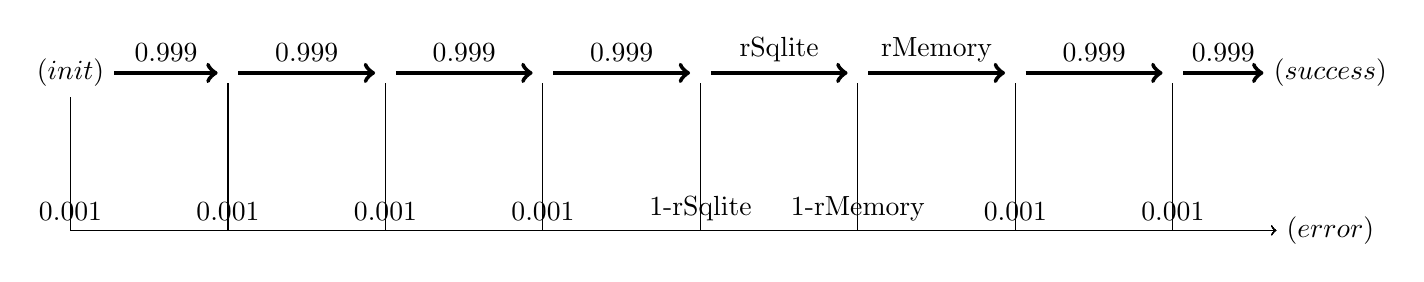
\begin{tikzpicture}[thick]
%\draw[help lines, step=1cm] (0,0) grid +(10,15);
%%%%%%%%%%%%%%%%%%%%%%%%%%%%%%% FDTMC for Oxygenation / Temperature
\node(init) at (0,7){$(init)$};
\node(s1) at (2,7){};
\node(s2) at (4,7){};
\node(s3) at (6,7){};
\node(s4) at (8,7){};
\node(s5) at (10,7){};
\node(s6) at (12,7){};
\node(s7) at (14,7){};
\node(success) at (16,7){$(success)$};
\node(error) at (16,5){$(error)$};
\draw[->, ultra thick] (init) -- node[draw=none, above]{0.999}(s1);
\draw[->, ultra thick] (s1) -- node[draw=none, above]{0.999}(s2);
\draw[->, ultra thick] (s2) -- node[draw=none, above]{0.999}(s3);
\draw[->, ultra thick] (s3) -- node[draw=none, above]{0.999}(s4);
\draw[->, ultra thick] (s4) -- node[draw=none, above]{rSqlite}(s5);
\draw[->, ultra thick] (s5) -- node[draw=none, above]{rMemory}(s6);
\draw[->, ultra thick] (s6) -- node[draw=none, above]{0.999}(s7);
\draw[->, ultra thick] (s7) -- node[draw=none, above]{0.999}(success);
\draw[->,auto, thin] (init) |- node[draw=none, above]{0.001}(error);
\draw[->,auto, thin] (s1) |- node[draw=none, above]{0.001}(error);
\draw[->,auto, thin] (s2) |- node[draw=none, above]{0.001}(error);
\draw[->,auto, thin] (s3) |- node[draw=none, above]{0.001}(error);
\draw[->,auto, thin] (s4) |- node[draw=none, above]{1-rSqlite}(error);
\draw[->,auto, thin] (s5) |- node[draw=none, above]{1-rMemory}(error);
\draw[->,auto, thin] (s6) |- node[draw=none, above]{0.001}(error);
\draw[->,auto, thin] (s7) |- node[draw=none, above]{0.001}(error);
\end{tikzpicture}
}
	\caption{FDTMC of the \emph{Oxygenation} and \emph{Temperature} sequence diagrams}
	\label{fig:fdtmcOxygenationTemperature}
\end{figure}

In the case of the reliability analysis by employing a parametric model checker, the transformation rules represented by Figures~\ref{fig:transSync_SD} and \ref{fig:transOptFrag_SD} were applied to build the FDTMC related to the \texttt{rOxygenation} fragment. The resulting FDTMC is show by Figure~\ref{fig:fdtmcOxygenationTemperature} where the unique path leading to the $success$ stated is represented in bold. When the property $P_{=?}(\Diamond''success'')$ is evaluated by a parametric model checker's algorithm, it results into the formula $0.999^6 \times rSqlite \times rMemory$, where \texttt{rSqlite} and \texttt{rMemory} variables represent the reliabilities its related fragments may assume. Thus, both reliability formulae computed from the UML behavioral diagram and from the FDTMC are equal which brings evidences that reliability equivalence also holds for sequence diagrams. Such evidences are important to demonstrate that the semantics of UML sequence diagrams were preserved by their transformation rules to FDTMC sub-structures, in special, the transformation rule for the optional combined fragment (cf. Figure \ref{fig:transOptFrag_SD}) that was adapted to address the variability of software product lines.



%%%%%%%%%%%%%%%%%%%%%%%%%%%%%%%%%%%%%%%%%%%%%%%%%%%%%%%%%%%%%%%%%%%%%%%%%%%%%%%%
%% CONCLUSION
%%%%%%%%%%%%%%%%%%%%%%%%%%%%%%%%%%%%%%%%%%%%%%%%%%%%%%%%%%%%%%%%%%%%%%%%%%%%%%%%
\section{Conclusion \label{sec:modelingConclusion}}

In short, this chapter presented how the probabilistic and variable behavior of
a software product line can be represented by UML behavioral diagrams endowed
with probabilities on its elements. For each behavioral element used to
represent the software product line behavior a translation rule was defined in
order to allow creating the FDTMC for activity or sequence diagrams. The chapter
also defined the reliability notion of UML behavioral models for software
product lines which, to the best of our knowledge, was not defined yet. Finally,
some evidences for the reliability equivalence of both UML behavioral models and
their respective FDTMCs. 

Overall, the reliability function defined for UML behavioral diagrams operate
over the scope of the behavioral diagram under analysis. So each element defined
in a behavioral diagram will be considered as a term of the reliability
function, not mattering if the element comprises another behavioral element.
Such characteristic is plain when the reliability function operates over
activities comprising an activity diagram and combined fragments of sequence
diagrams (except the \texttt{loop}). In both cases the reliability is
represented by an variable representing the reliability of its associated
sequence diagram. 









